% ============================================================================
%  Chapitre 4 : Simulation de la sphère de Chaplygin
%  Une partie par fichier, incluses dans l'ordre.
% ============================================================================
\chapter{Simulation de la sphère de Chaplygin}

% Repère provisoire pour les parties à rédiger (à retirer à la fin)
\newcommand{\arediger}[1]{{\color{gray}\itshape À rédiger : #1}}

% ============================================================================
%  Chapitre 4, partie I : Dynamique par blocs de matrices
%  Matériau déjà rédigé : chapitre4/brouillon_blocs.tex
% ============================================================================

% ----------------------------------------------------------------------------
\section{Dynamique par blocs de matrices}
% ----------------------------------------------------------------------------

% ----------------------------------------------------------------------------
\subsection{Position du problème}

Simuler la sphère, c'est retrouver $q(t) = (r(t),\alpha(t))$ le long de
la trajectoire, où $r = (x,y)$ est la position de $G$ dans le plan et
$\alpha = (\varphi,\theta,\psi)$ l'orientation de la sphère. Cependant, avec le principe d'Alembert, on a deux inconnues qui interviennent en plus
$\vect{\lambda} = (\lambda_1,\lambda_2)$. On a donc
$5 + 2 = 7$ inconnues, pour $5$ équations
d'Euler-Lagrange-d'Alembert et $2$ équations de contrainte.

Ces deux familles d'équations ne sont pas de même nature : les
premières sont du second ordre en $q$, les secondes du premier ordre,
et $\vect{\lambda}$ n'y apparaît jamais dérivé. On ne peut donc pas les
intégrer directement. L'idée est de chercher, à chaque instant, un
système qui détermine $(\ddot q,\vect{\lambda})$ à partir de
$(q,\dot q)$ : il suffit ensuite d'intégrer $\ddot q$ dans le temps
pour obtenir $q(t)$.

% ----------------------------------------------------------------------------
\subsection{Forme générale}

On considère un lagrangien de la forme
\[
    L(q,\dot q) = \tfrac12\,\dot q^T\mat{M}(q)\,\dot q - V(q)
\]
où $\mat{M}(q) = \partial^2 T/\partial\dot q^2$ est la matrice de
masse, symétrique définie positive. C'est la version matricielle de
l'exemple scalaire du chapitre 1. Comme $\mat{M}$ est symétrique,
\[
    \pd{L}{\dot q} = \mat{M}\,\dot q
    \longrightarrow
    \ddt\pd{L}{\dot q} = \mat{M}\,\ddot q + \dot{\mat{M}}\,\dot q,
    \qquad
    \pd{L}{q} = \tfrac12\,\nabla_q\bigl(\dot q^T\mat{M}\,\dot q\bigr)
    - \nabla V
\]
où $\dot{\mat{M}} = \sum_k \pd{\mat{M}}{q_k}\,\dot q_k$. Les équations
d'Euler-Lagrange-d'Alembert, sans force non conservative, deviennent
\[
    \mat{M}(q)\,\ddot q + \vect{h}(q,\dot q) + \nabla V(q)
    = \mat{A}(q)^T\vect{\lambda},
    \qquad
    \vect{h} = \dot{\mat{M}}\,\dot q
    - \tfrac12\,\nabla_q\bigl(\dot q^T\mat{M}\,\dot q\bigr)
\]
où $\vect{h}$ regroupe les termes quadratiques en $\dot q$. Pour la
sphère de Chaplygin, $V = m g a$ est constant, donc $\nabla V = 0$.

Ces $5$ équations sont linéaires en $(\ddot q,\vect{\lambda})$, mais
il en faut $7$. La contrainte $\mat{A}(q)\,\dot q = 0$ ne fait pas
intervenir $\ddot q$ donc on la dérive par rapport au temps pour obtenir
deux équations en $\ddot q$,
\[
    \mat{A}(q)\,\ddot q + \dot{\mat{A}}\,\dot q = 0,
    \qquad
    \dot{\mat{A}} = \sum_k \pd{\mat{A}}{q_k}\,\dot q_k
\]

\begin{proposition}[Système par blocs]
    Si la contrainte est vérifiée à l'instant initial, les équations
    d'Euler-Lagrange-d'Alembert et la contrainte équivalent au système
    \[
        \begin{pmatrix}
            \mat{M}(q) & -\,\mat{A}(q)^T\\
            \mat{A}(q) & \mat{0}
        \end{pmatrix}
        \begin{pmatrix}
            \ddot q\\ \vect{\lambda}
        \end{pmatrix}
        = \begin{pmatrix}
            -\,\vect{h}(q,\dot q) - \nabla V(q)\\
            -\,\dot{\mat{A}}\,\dot q
        \end{pmatrix}
    \]
    Si $\mat{M}(q)$ est symétrique définie positive et si
    $\mat{A}(q)$ est de rang maximal, la matrice du système est
    inversible : $(q,\dot q)$ permet donc de déterminer $(\ddot q,\vect{\lambda})$.
\end{proposition}

Pour simuler la sphère, il reste donc à calculer les blocs
$\mat{M}$, $\vect{h}$, $\mat{A}$ et $\dot{\mat{A}}\,\dot q$.

% ----------------------------------------------------------------------------
\subsection{Séparation translation et orientation}

On sépare la position de $G$ dans le plan et l'orientation de la
sphère :
\[
    q = (r,\alpha),
    \qquad
    r = (x,y),
    \qquad
    \alpha = (\varphi,\theta,\psi)
\]
D'après le chapitre 3 (I.4.3), la vitesse angulaire dans $\rep{s}$
s'écrit $\vect{\Omega} = \mat{E}_s(\alpha)\,\dot\alpha$, où
$\mat{E}_s$ est la matrice de la convention d'Euler $Z$-$Y'$-$X''$. Dans le
corps, $\vect{\omega} = \mat{R}^T\vect{\Omega}$, donc
\[
    \vect{\omega} = \mat{E}(\alpha)\,\dot\alpha,
    \qquad 
    \text{avec} \quad
    \mat{E} = \mat{R}^T\mat{E}_s
    = \begin{pmatrix}
        1 & 0 & -s_\theta\\
        0 & c_\varphi & s_\varphi c_\theta\\
        0 & -s_\varphi & c_\varphi c_\theta
    \end{pmatrix}
\]
avec $\det\mat{E} = \cos\theta$. De même, la contrainte
$\mat{A}(q)\,\dot q = 0$ se découpe selon $q = (r,\alpha)$ :
\[
    \mat{A} = \begin{pmatrix} \Id_2 & \mat{A}_\alpha(\alpha)
    \end{pmatrix}
    \longleftrightarrow
    \dot r + \mat{A}_\alpha\,\dot\alpha = 0
\]
\begin{remarque}
    Lorsque le pitch $\theta = \pm \frac{\pi}{2}$, on aura la dégénéresance, et le système n'est plus solvable. Ainsi, pour la simulation numérique, il faut encoder 
    l'orientation par quaternion.
\end{remarque}
% ----------------------------------------------------------------------------
\subsection{Calcul des blocs}

\subsubsection{Matrice de masse}

D'après le théorème de König, avec
$\vect{\omega} = \mat{E}(\alpha)\,\dot\alpha$,
\[
    T = \tfrac12\,m\,\dot r^T\dot r
    + \tfrac12\,\vect{\omega}^T\mat{I}_b\,\vect{\omega}
    = \tfrac12\,m\,\dot r^T\dot r
    + \tfrac12\,\dot\alpha^T\mat{E}^T\mat{I}_b\,\mat{E}\,\dot\alpha
    = \tfrac12\,\dot q^T\mat{M}\,\dot q
\]
d'où la matrice de masse, diagonale par blocs,
\[
    \mat{M} = \begin{pmatrix}
        m\,\Id_2 & \mat{0}\\
        \mat{0} & \mat{M}_\alpha
    \end{pmatrix},
    \qquad
    \mat{M}_\alpha = \mat{E}^T\mat{I}_b\,\mat{E}
\]
Avec $\mat{I}_b = \mathrm{diag}(I_1,I_2,I_3)$ et l'expression de
$\mat{E}$,
\[
    \mat{M}_\alpha = \begin{pmatrix}
        I_1 & 0 & -I_1 s_\theta\\
        0 & I_2 c_\varphi^2 + I_3 s_\varphi^2
            & (I_2 - I_3)\,s_\varphi c_\varphi c_\theta\\
        -I_1 s_\theta & (I_2 - I_3)\,s_\varphi c_\varphi c_\theta
            & I_1 s_\theta^2 + (I_2 s_\varphi^2 + I_3 c_\varphi^2)\,
            c_\theta^2
    \end{pmatrix}
\]

\subsubsection{Termes quadratiques}

Comme $\mat{M}$ ne dépend que de $\alpha$, et pas de $r$, et que son
bloc $m\,\Id_2$ est constant, la partie de $\vect{h}$ en $r$ s'annule :
\[
    \vect{h} = \begin{pmatrix} \vect{0}\\ \vect{h}_\alpha \end{pmatrix},
    \qquad
    \vect{h}_\alpha = \dot{\mat{M}}_\alpha\,\dot\alpha
    - \tfrac12\,\nabla_\alpha\bigl(\dot\alpha^T\mat{M}_\alpha\,\dot\alpha\bigr)
\]
Ce calcul direct est lourd, car il faut dériver chaque coefficient de
$\mat{M}_\alpha$. On passe plutôt par $\vect{\omega}$. L'énergie de
rotation s'écrit
\[
    T_\alpha = \tfrac12\,\vect{\omega}^T\mat{I}_b\,\vect{\omega}
    = \tfrac12\,\dot\alpha^T\mat{M}_\alpha\,\dot\alpha,
    \qquad
    \vect{\omega} = \mat{E}(\alpha)\,\dot\alpha
\]
et, on a
$\ddt\pd{T_\alpha}{\dot\alpha} - \pd{T_\alpha}{\alpha}
= \mat{M}_\alpha\,\ddot\alpha + \vect{h}_\alpha$. Par la règle de chaîne,
\[
    \pd{T_\alpha}{\dot\alpha}
    = \Bigl(\pd{\vect{\omega}}{\dot\alpha}\Bigr)^T\mat{I}_b\,\vect{\omega}
    = \mat{E}^T\mat{I}_b\,\vect{\omega},
    \qquad
    \pd{T_\alpha}{\alpha}
    = \Bigl(\pd{\vect{\omega}}{\alpha}\Bigr)^T\mat{I}_b\,\vect{\omega}
\]
où $\pd{\vect{\omega}}{\alpha}$ est la jacobienne de $\vect{\omega}$
par rapport à $\alpha$, à $\dot\alpha$ fixé. On en déduit
\[
    \ddt\pd{T_\alpha}{\dot\alpha} - \pd{T_\alpha}{\alpha}
    = \mat{E}^T\mat{I}_b\,\dot{\vect{\omega}}
    + \Bigl(\dot{\mat{E}} - \pd{\vect{\omega}}{\alpha}\Bigr)^T
    \mat{I}_b\,\vect{\omega}
\]

On note $\vect{e}_j$ la $j$-ième colonne de
$\mat{E}$, $\partial_k = \partial/\partial\alpha_k$, pour la compacité, on va utiliser la notation d'Einstein. Alors
$\vect{\omega} = \vect{e}_k\,\dot\alpha_k$, et les $j$-ièmes colonnes
de $\dot{\mat{E}}$ et de $\pd{\vect{\omega}}{\alpha}$ sont
\[
    \dot{\mat{E}}_{\cdot j} = (\partial_k\vect{e}_j)\,\dot\alpha_k,
    \qquad
    \Bigl(\pd{\vect{\omega}}{\alpha}\Bigr)_{\!\cdot j}
    = \partial_j\bigl(\vect{e}_k\,\dot\alpha_k\bigr)
    = (\partial_j\vect{e}_k)\,\dot\alpha_k
\]
d'où
\[
    \Bigl(\dot{\mat{E}} - \pd{\vect{\omega}}{\alpha}\Bigr)_{\!\cdot j}
    = \bigl(\partial_k\vect{e}_j - \partial_j\vect{e}_k\bigr)\,
    \dot\alpha_k
\]

\begin{proposition}[Colonnes de $\mat{E}$]
    Pour tous $j,k$, les colonnes de $\mat{E}$ vérifient
    \[
        \partial_k\vect{e}_j - \partial_j\vect{e}_k
        = \vect{e}_j\wedge\vect{e}_k
    \]
\end{proposition}

\begin{demonstration}
    Par la règle de chaîne, $\dot{\mat{R}} = (\partial_k\mat{R})\,
    \dot\alpha_k$, et sachant que l'on a : $\vect{\omega} = \vect{e_k} \dot{\alpha}_k$, par linéarité on obtiendras $\hatx{\vect{\omega}} = \hatx{e_k \dot{\alpha}_k}$ d'où $\hatx{\vect{\omega}} = \hatx{\vect{e}_k}\,
    \dot\alpha_k$. La proposition 2.18 donne
    $(\mat{R}^T\partial_k\mat{R})\,\dot\alpha_k
    = \hatx{\vect{e}_k}\,\dot\alpha_k$ pour tout $\dot\alpha$, donc on a : 
    \[
        \partial_k\mat{R} = \mat{R}\,\hatx{\vect{e}_k}
    \]
    En dérivant par rapport à $\alpha_j$, puis en utilisant la relation que l'on vient d'obtenir on a : 
    \[
        \partial_j\partial_k\mat{R}
        = (\partial_j\mat{R})\,\hatx{\vect{e}_k}
        + \mat{R}\,\hatx{\partial_j\vect{e}_k}
        = \mat{R}\bigl(\hatx{\vect{e}_j}\hatx{\vect{e}_k}
        + \hatx{\partial_j\vect{e}_k}\bigr)
    \]
    D'après le théorème de Schwarz, on a
    $\partial_j\partial_k\mat{R} = \partial_k\partial_j\mat{R}$, donc
    \[
        \begin{aligned}
            &\partial_{jk}\mat{R} - \partial_{kj}\mat{R} = \mat{0}\\
            \longleftrightarrow\;
            &\mat{R}\bigl(\hatx{\vect{e}_j}\hatx{\vect{e}_k}
            + \hatx{\partial_j\vect{e}_k}\bigr)
            - \mat{R}\bigl(\hatx{\vect{e}_k}\hatx{\vect{e}_j}
            + \hatx{\partial_k\vect{e}_j}\bigr) = \mat{0}
        \end{aligned}
    \]

    Comme les indices $j$ et $k$ sont arbitraires, $\partial_{kj}\mat{R}$
    s'obtient en échangeant $j$ et $k$ dans l'expression de
    $\partial_{jk}\mat{R}$. En simplifiant par $\mat{R}$ inversible
    ($\mat{R}^{-1} = \mat{R}^T$), on obtient alors :
    \[
        \hatx{\partial_k\vect{e}_j - \partial_j\vect{e}_k}
        = \hatx{\vect{e}_j}\hatx{\vect{e}_k}
        - \hatx{\vect{e}_k}\hatx{\vect{e}_j}
    \]
    Enfin, pour tout $\vect{w}$, avec le double produit vectoriel,
    \[
        \begin{aligned}
            \bigl(\hatx{\vect{u}}\hatx{\vect{v}}
            - \hatx{\vect{v}}\hatx{\vect{u}}\bigr)\vect{w}
            &= \vect{u}\wedge(\vect{v}\wedge\vect{w})
            - \vect{v}\wedge(\vect{u}\wedge\vect{w})\\
            &= \vect{v}\,(\vect{u}\cdot\vect{w})
            - \vect{w}\,(\vect{u}\cdot\vect{v})
            - \vect{u}\,(\vect{v}\cdot\vect{w})
            + \vect{w}\,(\vect{v}\cdot\vect{u})\\
            &= \vect{v}\,(\vect{u}\cdot\vect{w})
            - \vect{u}\,(\vect{v}\cdot\vect{w})
            = (\vect{u}\wedge\vect{v})\wedge\vect{w}
        \end{aligned}
    \]
    donc $\hatx{\vect{u}}\hatx{\vect{v}} - \hatx{\vect{v}}\hatx{\vect{u}}
    = \hatx{\vect{u}\wedge\vect{v}}$.
\end{demonstration}

D'après cette proposition, la $j$-ième colonne de
$\dot{\mat{E}} - \pd{\vect{\omega}}{\alpha}$ vaut
\[
    \Bigl(\dot{\mat{E}} - \pd{\vect{\omega}}{\alpha}\Bigr)_{\!\cdot j}
    = (\vect{e}_j\wedge\vect{e}_k)\,\dot\alpha_k
    = \vect{e}_j\wedge(\vect{e}_k\,\dot\alpha_k)
    = \vect{e}_j\wedge\vect{\omega}
\]
La $j$-ième composante de
$\bigl(\dot{\mat{E}} - \pd{\vect{\omega}}{\alpha}\bigr)^T
\mat{I}_b\,\vect{\omega}$ est donc un produit mixte :
\[
    (\vect{e}_j\wedge\vect{\omega})\cdot\mat{I}_b\,\vect{\omega}
    = \det\bigl(\vect{e}_j,\vect{\omega},\mat{I}_b\,\vect{\omega}\bigr)
\]

Ici, on fait une permutation paire ($1 \leftrightarrow 3 \longrightarrow 1 \leftrightarrow 2$), ce qui ne change pas le déterminant : 
\[
    \det\bigl(\vect{e}_j,\vect{\omega},\mat{I}_b\,\vect{\omega}\bigr)
    = \det\bigl(\vect{\omega},\mat{I}_b\,\vect{\omega},\vect{e}_j\bigr)
    = \vect{e}_j\cdot\bigl(\vect{\omega}\wedge(\mat{I}_b\,\vect{\omega})\bigr)
\]
Puisque $\vect{e}_j$ est la $j$-ième colonne de $\mat{E}$,
$\vect{e}_j\cdot\vect{v}$ est la $j$-ième composante de
$\mat{E}^T\vect{v}$, d'où

\[
    \Bigl(\dot{\mat{E}} - \pd{\vect{\omega}}{\alpha}\Bigr)^T
    \mat{I}_b\,\vect{\omega}
    = \mat{E}^T\bigl(\vect{\omega}\wedge(\mat{I}_b\,\vect{\omega})\bigr)
\]
On retrouve ici le terme gyroscopique
$\vect{\omega}\wedge(\mat{I}_b\,\vect{\omega})$.

On calcule le premier terme. En dérivant $\vect{\omega} = \mat{E}\,\dot\alpha$,
on a $\dot{\vect{\omega}} = \mat{E}\,\ddot\alpha + \dot{\mat{E}}\,\dot\alpha$,
donc
\[
    \mat{E}^T\mat{I}_b\,\dot{\vect{\omega}}
    = \mat{E}^T\mat{I}_b\,\mat{E}\,\ddot\alpha
    + \mat{E}^T\mat{I}_b\,\dot{\mat{E}}\,\dot\alpha
    = \mat{M}_\alpha\,\ddot\alpha
    + \mat{E}^T\mat{I}_b\,\dot{\mat{E}}\,\dot\alpha
\]
En rassemblant les deux termes, on a
\[
    \ddt\pd{T_\alpha}{\dot\alpha} - \pd{T_\alpha}{\alpha}
    = \mat{M}_\alpha\,\ddot\alpha
    + \mat{E}^T\bigl(\mat{I}_b\,\dot{\mat{E}}\,\dot\alpha
    + \vect{\omega}\wedge(\mat{I}_b\,\vect{\omega})\bigr)
\]
et, par identification avec $\mat{M}_\alpha\,\ddot\alpha + \vect{h}_\alpha$,
on déduit : 

\begin{proposition}[Termes quadratiques]
    Le terme quadratique du modèle de simulation de la sphère de Chaplygin est
    \[
        \vect{h} = \begin{pmatrix} \vect{0}\\ \vect{h}_\alpha \end{pmatrix},
        \qquad
        \vect{h}_\alpha = \mat{E}^T\bigl(\mat{I}_b\,\dot{\mat{E}}\,\dot\alpha
        + \vect{\omega}\wedge(\mat{I}_b\,\vect{\omega})\bigr),
        \qquad
        \vect{\omega} = \mat{E}\,\dot\alpha
    \]
\end{proposition}

\subsubsection{Contrainte}

D'après la forme matricielle de la contrainte que l'on a obtenue en chapitre 3, le bloc
d'orientation de $\mat{A} = \begin{pmatrix} \Id_2 & \mat{A}_\alpha
\end{pmatrix}$ est
\[
    \mat{A}_\alpha = a\begin{pmatrix}
        -s_\psi c_\theta & -c_\psi & 0\\
        c_\psi c_\theta & -s_\psi & 0
    \end{pmatrix}
\]
Le bloc $\Id_2$ est constant, donc
$\dot{\mat{A}}\,\dot q = \dot{\mat{A}}_\alpha\,\dot\alpha$. Comme
$\mat{A}_\alpha$ ne dépend que de $\theta$ et $\psi$,
$\dot{\mat{A}}_\alpha = \partial_\theta\mat{A}_\alpha\,\dot\theta
+ \partial_\psi\mat{A}_\alpha\,\dot\psi$, soit
\[
    \dot{\mat{A}}_\alpha = a\begin{pmatrix}
        -\dot\psi\,c_\psi c_\theta + \dot\theta\,s_\psi s_\theta
            & \dot\psi\,s_\psi & 0\\
        -\dot\psi\,s_\psi c_\theta - \dot\theta\,c_\psi s_\theta
            & -\dot\psi\,c_\psi & 0
    \end{pmatrix}
\]
d'où
\[
    \dot{\mat{A}}_\alpha\,\dot\alpha = a\begin{pmatrix}
        -\dot\varphi\dot\psi\,c_\psi c_\theta
        + \dot\varphi\dot\theta\,s_\psi s_\theta
        + \dot\theta\dot\psi\,s_\psi\\
        -\dot\varphi\dot\psi\,s_\psi c_\theta
        - \dot\varphi\dot\theta\,c_\psi s_\theta
        - \dot\theta\dot\psi\,c_\psi
    \end{pmatrix}
\]

% ----------------------------------------------------------------------------
\subsection{Système par blocs de la sphère}

On rassemblent alors les blocs du système, en séparant le mouvement translationnel et l'orientation et contraintes, on a avec $q = (r,\alpha)$ et
$\mat{A}^T\vect{\lambda} = (\vect{\lambda},\,\mat{A}_\alpha^T\vect{\lambda})$ : 

\begin{theoreme}[Modèle de simulation de la sphère de Chaplygin]
    Tant que $\cos\theta \neq 0$, l'état $(r,\alpha,\dot r,\dot\alpha)$
    détermine de manière unique $(\ddot r,\ddot\alpha,\vect{\lambda})$,
    solution de
    \[
        \begin{pmatrix}
            m\,\Id_2 & \mat{0} & -\,\Id_2\\
            \mat{0} & \mat{M}_\alpha & -\,\mat{A}_\alpha^T\\
            \Id_2 & \mat{A}_\alpha & \mat{0}
        \end{pmatrix}
        \begin{pmatrix}
            \ddot r\\ \ddot\alpha\\ \vect{\lambda}
        \end{pmatrix}
        = \begin{pmatrix}
            \vect{0}\\
            -\,\vect{h}_\alpha\\
            -\,\dot{\mat{A}}_\alpha\,\dot\alpha
        \end{pmatrix}
    \]
    avec $\mat{M}_\alpha = \mat{E}^T\mat{I}_b\,\mat{E}$,
    $\vect{h}_\alpha = \mat{E}^T\bigl(\mat{I}_b\,\dot{\mat{E}}\,\dot\alpha
    + \vect{\omega}\wedge(\mat{I}_b\,\vect{\omega})\bigr)$,
    $\vect{\omega} = \mat{E}\,\dot\alpha$, et $\mat{A}_\alpha$,
    $\dot{\mat{A}}_\alpha\,\dot\alpha$ donnés en 4.3.
\end{theoreme}

% ----------------------------------------------------------------------------
\subsection{Système réduit}

Apparemment, le système a 7 inconnues, mais on peut voir directement dans le théorème ci-dessus que la troisième ligne donne directement $\ddot{r}$ et la première ligne donne ensuite $\vect{\lambda}$, les deux en fonction de $\alpha$ : 
\[
    \ddot r = -\,\bigl(\mat{A}_\alpha\,\ddot\alpha
    + \dot{\mat{A}}_\alpha\,\dot\alpha\bigr),
    \qquad
    \vect{\lambda} = m\,\ddot r
    = -\,m\,\bigl(\mat{A}_\alpha\,\ddot\alpha
    + \dot{\mat{A}}_\alpha\,\dot\alpha\bigr)
\]
En reportant $\vect{\lambda}$ dans la deuxième ligne,
$\mat{M}_\alpha\,\ddot\alpha + \vect{h}_\alpha
= -\,m\,\mat{A}_\alpha^T\bigl(\mat{A}_\alpha\,\ddot\alpha
+ \dot{\mat{A}}_\alpha\,\dot\alpha\bigr)$, d'où le résultat suivant : 

\begin{corollaire}[Système réduit]
    Tant que $\cos\theta \neq 0$, l'orientation vérifie
    \[
        \bigl(\mat{M}_\alpha + m\,\mat{A}_\alpha^T\mat{A}_\alpha\bigr)\,
        \ddot\alpha
        = -\,\vect{h}_\alpha
        - m\,\mat{A}_\alpha^T\dot{\mat{A}}_\alpha\,\dot\alpha
    \]
    et la position et les réactions s'en déduisent par
    \[
        \dot r = -\,\mat{A}_\alpha\,\dot\alpha,
        \qquad
        \ddot r = -\,\bigl(\mat{A}_\alpha\,\ddot\alpha
        + \dot{\mat{A}}_\alpha\,\dot\alpha\bigr),
        \qquad
        \vect{\lambda} = m\,\ddot r
    \]
\end{corollaire}

On n'intègre donc que $\alpha$, système $3\times3$ au lieu de $7\times7$,
et la contrainte $\dot r = -\,\mat{A}_\alpha\,\dot\alpha$ est vérifiée
par construction. La matrice
$\mat{M}_\alpha + m\,\mat{A}_\alpha^T\mat{A}_\alpha$ est l'inertie
autour du point de contact $P$ : avec $\vect{\Omega} = \mat{E}_s\,\dot\alpha$,
\[
    \mat{M}_\alpha + m\,\mat{A}_\alpha^T\mat{A}_\alpha
    = \mat{E}_s^T\,\mat{I}_P\,\mat{E}_s,
    \qquad
    \mat{I}_P = \mat{I}_G + m\,a^2\bigl(\Id - \vect{e}_z\vect{e}_z^T\bigr)
\]
où $\mat{I}_G = \mat{R}\,\mat{I}_b\,\mat{R}^T$, d'après le théorème de
Huygens-Steiner avec $\overrightarrow{GP} = -\,a\,\vect{e}_z$.
   % I. Dynamique par blocs de matrices

% ============================================================================
%  Chapitre 4, partie II : Algorithme de simulation
% ============================================================================

% ----------------------------------------------------------------------------
\section{Algorithme de simulation - Orientation en angles d'Euler}
% ----------------------------------------------------------------------------
On peut se demander pourquoi on effectue une simulation avec les angles
d'Euler pour décrire l'orientation, alors que l'on abandonne cette
piste juste après : la simulation ne tient que tant que
$|\cos\theta| > \varepsilon$. La raison est simple : c'est la
traduction directe de tout ce que l'on a développé auparavant. Cette
simulation montre ce que donne la dynamique : la trajectoire de $G$,
les angles, les réactions. L'interprétation des quaternions, en
revanche, n'est pas directe, et intuitive et cette simulation permet donc de fixer
ce que l'on attend du simulateur en quaternions. C'est pourquoi on ne
fait pas, dans cette partie, d'analyse de convergence détaillée.
% ----------------------------------------------------------------------------
\subsection{Système global}

On note $\mat{K}_\alpha = \mat{M}_\alpha + m\,\mat{A}_\alpha^T\mat{A}_\alpha$.
D'après le corollaire 4.6, l'état $(r,\alpha,\dot\alpha)$ vérifie le
système du premier ordre
\[
    \ddt\begin{pmatrix} r\\ \alpha\\ \dot\alpha \end{pmatrix}
    = \begin{pmatrix}
        -\,\mat{A}_\alpha\,\dot\alpha\\
        \dot\alpha\\
        \mat{K}_\alpha^{-1}\bigl(-\,\vect{h}_\alpha
        - m\,\mat{A}_\alpha^T\dot{\mat{A}}_\alpha\,\dot\alpha\bigr)
    \end{pmatrix}
\]
Les deux dernières lignes ne dépendent pas de $r$. On résout donc
d'abord $(\alpha,\dot\alpha)$ seul, puis on en déduit $r$ et
$\vect{\lambda}$.

% ----------------------------------------------------------------------------
\subsection{Sous-système en orientation}

\begin{proposition}[Sous-système en orientation]
    On pose $Y = (\alpha,\dot\alpha)$, qui vérifie
\[
    \dot Y = f(Y) = \begin{pmatrix} \dot\alpha\\ \ddot\alpha \end{pmatrix},
    \qquad
    \mat{K}_\alpha\,\ddot\alpha = -\,\vect{h}_\alpha
    - m\,\mat{A}_\alpha^T\dot{\mat{A}}_\alpha\,\dot\alpha
\]
\end{proposition}
On peut résoudre numériquement ce système avec les conditions initiales de $\alpha$ et $\dot{\alpha}$, ce qui permet de calculer $\ddot{\alpha}$ par résolution d'un système d'équations. Ensuite, une fois obtenu ces trois informations, on peut calculer la position de centre de masse et les forces de réaction.

% ----------------------------------------------------------------------------
\subsection{Sous-système en position et réactions}

\begin{proposition}[Sous-système en position et réactions]
    Une fois $(\alpha,\dot\alpha,\ddot\alpha)$ connu, le reste se calcule facilement : 
\[
    \dot r = -\,\mat{A}_\alpha\,\dot\alpha,
    \qquad
    \vect{\lambda} = -\,m\,\bigl(\mat{A}_\alpha\,\ddot\alpha
    + \dot{\mat{A}}_\alpha\,\dot\alpha\bigr)
\]
\end{proposition}


% ----------------------------------------------------------------------------
\subsection{Schéma de Runge-Kutta d'ordre 4 (RK4) pour la résolution de la dynamique}

\subsubsection{Schéma RK4}

Pour $\dot Y = f(Y)$, avec un pas $h$ et $Y_k \approx Y(t_k)$,
$t_k = k\,h$,
\[
    \begin{aligned}
        \vect{p}_1 &= f(Y_k), &
        \vect{p}_2 &= f\bigl(Y_k + \tfrac{h}{2}\,\vect{p}_1\bigr),\\
        \vect{p}_3 &= f\bigl(Y_k + \tfrac{h}{2}\,\vect{p}_2\bigr), &
        \vect{p}_4 &= f\bigl(Y_k + h\,\vect{p}_3\bigr)
    \end{aligned}
    \qquad
    Y_{k+1} = Y_k + \tfrac{h}{6}\,\bigl(\vect{p}_1 + 2\,\vect{p}_2
    + 2\,\vect{p}_3 + \vect{p}_4\bigr)
\]
L'erreur est en $O(h^5)$ sur un pas et en $O(h^4)$ sur un intervalle
fixé.

\subsubsection{Schéma RK4 pour simuler le système}

On se donne la condition initiale $(r_0,\alpha_0,\dot\alpha_0)$, avec
$\cos\theta_0 \neq 0$.

\paragraph{Étape 1 : orientation.} Avec $Y_k = (\alpha_k,\dot\alpha_k)$,
on évalue $f$ en quatre états intermédiaires du pas,
\[
    Y^{(1)} = Y_k,
    \qquad
    Y^{(2)} = Y_k + \tfrac{h}{2}\,\vect{p}_1,
    \qquad
    Y^{(3)} = Y_k + \tfrac{h}{2}\,\vect{p}_2,
    \qquad
    Y^{(4)} = Y_k + h\,\vect{p}_3
\]
où $Y^{(i)} = (\alpha^{(i)},\dot\alpha^{(i)})$ et
\[
    \vect{p}_i = f\bigl(Y^{(i)}\bigr)
    = \begin{pmatrix} \dot\alpha^{(i)}\\ \ddot\alpha^{(i)} \end{pmatrix},
    \qquad
    \mat{K}_\alpha\bigl(\alpha^{(i)}\bigr)\,\ddot\alpha^{(i)}
    = -\,\vect{h}_\alpha\bigl(\alpha^{(i)},\dot\alpha^{(i)}\bigr)
    - m\,\mat{A}_\alpha^T\dot{\mat{A}}_\alpha\,\dot\alpha\,\big|^{(i)}
\]
On obtient alors le nouvel état $Y_{k+1} = (\alpha_{k+1},\dot\alpha_{k+1})$ :
\[
    \alpha_{k+1} = \alpha_k + \tfrac{h}{6}\,\bigl(\dot\alpha^{(1)}
    + 2\,\dot\alpha^{(2)} + 2\,\dot\alpha^{(3)} + \dot\alpha^{(4)}\bigr),
    \qquad
    \dot\alpha_{k+1} = \dot\alpha_k + \tfrac{h}{6}\,\bigl(\ddot\alpha^{(1)}
    + 2\,\ddot\alpha^{(2)} + 2\,\ddot\alpha^{(3)} + \ddot\alpha^{(4)}\bigr)
\]

\paragraph{Étape 2 : accélération.} On résout le système réduit au
nouvel état :
\[
    \mat{K}_\alpha(\alpha_{k+1})\,\ddot\alpha_{k+1}
    = -\,\vect{h}_\alpha(\alpha_{k+1},\dot\alpha_{k+1})
    - m\,\mat{A}_\alpha^T\dot{\mat{A}}_\alpha\,\dot\alpha\,\big|_{k+1}
\]
C'est la seconde moitié de $f(Y_{k+1})$, réutilisée comme $\vect{p}_1$
au pas suivant.

\paragraph{Étape 3 : position et réactions.} En parallèle avec étape 1, on calcule des poids RK4 pour $r$ avec 
$\vect{g}_i = -\,\mat{A}_\alpha\bigl(\alpha^{(i)}\bigr)\,
\dot\alpha^{(i)}$ tels que : 
\[
    r_{k+1} = r_k + \tfrac{h}{6}\,\bigl(\vect{g}_1 + 2\,\vect{g}_2
    + 2\,\vect{g}_3 + \vect{g}_4\bigr),
    \qquad
    \vect{\lambda}_{k+1} = -\,m\,\bigl(\mat{A}_\alpha(\alpha_{k+1})\,
    \ddot\alpha_{k+1}
    + \dot{\mat{A}}_\alpha\,\dot\alpha\,\big|_{k+1}\bigr)
\]


% ----------------------------------------------------------------------------
\subsection{Conditions initiales et choix du pas}

\subsubsection{Conditions initiales}
\begin{proposition}[Conditions initiales]
    Les conditions initiales de cette dynamique sont $(r_0, \alpha_0, \dot{\alpha}_0)$.
\end{proposition}

On choisit librement la position $r_0$, l'orientation $\alpha_0$ avec
$\cos\theta_0 \neq 0$, et les vitesses angulaires $\dot\alpha_0$. En
pratique, on se donne plutôt la vitesse angulaire $\vect{\Omega}_0$ dans
$\rep{s}$ et
\[
    \dot\alpha_0 = \mat{E}_s(\alpha_0)^{-1}\,\vect{\Omega}_0,
    \qquad
    \det\mat{E}_s = \cos\theta_0 \neq 0
\]
\begin{remarque}[Sur les vitesses angulaires]
    On peut aussi se donner la vitesse angulaire $\vect{\omega}_0$
    dans le repère corps. Cependant, on préfère le repère sol, car ses axes sont fixes et visuels et chaque composante de $\vect{\Omega}_0$ a un sens direct :
    $\Omega_x$ et $\Omega_y$ fixent le roulement initial,
    $\dot r_0 = a\,(\Omega_y, -\Omega_x)$, et $\Omega_z$ la rotation
    autour de la verticale. Les axes du corps, selon nos conventions, sont les axes principaux d'inertie :
    ils dépendent de la répartition de masse à l'intérieur de la
    sphère, et il est difficile de les repérer visuellement.
\end{remarque}

Par contre, la vitesse de $G$ n'est pas libre, le roulement impose
$\dot r_0 = -\,\mat{A}_\alpha(\alpha_0)\,\dot\alpha_0$. Enfin,
$\ddot\alpha_0$ et $\vect{\lambda}_0$ s'obtiennent directement en faisant les mêmes calculs que l'étape 2.

\subsubsection{Choix du pas}

\textbf{A discuter !!!!!}
Il faut noter qu'avec la modélisation en angles d'Euler, les conditionnements de notre système s'explose lorsqu'on a gimbal lock.

% ----------------------------------------------------------------------------
\subsection{Contrôle de la simulation}

Le schéma ne garantit pas la physique : on contrôle après coup que la
trajectoire calculée respecte ce que le modèle impose.

\subsubsection{Quantités conservées}

Ni le poids ni la force de réaction travaille, l'énergie cinétique doit rester donc constante.
\[
    T = \tfrac12\,m\,\dot r^T\dot r
    + \tfrac12\,\vect{\omega}^T\mat{I}_b\,\vect{\omega}
\]
est conservée. 

De plus, la réaction s'applique en $P$ et le poids passe
par $P$, leur moment en $P$ est nul, donc le moment cinétique au point
de contact 
\[
    \vect{L}_P = \mat{I}_P\,\vect{\Omega},
    \qquad
    \mat{I}_P = \mat{I}_G + m\,a^2\bigl(\Id - \vect{e}_z\vect{e}_z^T\bigr) = \mat{R} \mat{I}_b \mat{R} ^T + m\,a^2\bigl(\Id - \vect{e}_z\vect{e}_z^T\bigr)
\]
doit être conservé dans $\rep{s}$.

\begin{remarque}[Racine de l'anomalie de trajectoire de la sphère de Chaplygin]
    On a ici que $\vect{L}_P = \mat{I}_P \vect{\Omega}$ est conservée donc $\vect{\Omega} = \mat{I}_P ^{-1} \vect{cte}$ ou $\vect{\Omega} = {(\mat{R} \mat{I}_b \mat{R} ^T + m\,a^2\bigl(\Id - \vect{e}_z\vect{e}_z^T\bigr) )}^{-1}\vect{cte}$. Pour une sphère isotrope, $\mat{I}_P$ ne dépend pas de $\mat{R}$, donc $\vect{\Omega}$ reste une constante au long de la trajectoire, alors que si la sphère est anisotrope, $\mat{I}_P$ dépend de $\mat{R}(t)$, donc $\vect{\Omega}$ varie au long de la trajectoire. 

    D'un autre point de vue, si la sphère est isotrope ($\mat{I}_b = i\,\Id$),
    le terme gyroscopique $\vect{\omega}\wedge(\mat{I}_b\vect{\omega})$ est nul,
    $\mat{I}_P$ ne dépend pas de l'orientation et $\vect{\Omega}$ reste constant,
    la sphère roule ainsi en ligne droite. Sinon, le terme gyroscopique est non nul :
    $\vect{L}_P$ reste fixe dans $\rep{s}$ alors que l'inertie tourne avec le
    corps, donc $\vect{\omega}$ se réoriente dans $\rep{b}$, et $\vect{\Omega}$,
    puis la direction de $\dot{r}$.
\end{remarque}
On suit les dérives relatives
\[
    \frac{|T(t_k) - T(0)|}{T(0)},
    \qquad
    \frac{\|\vect{L}_P(t_k) - \vect{L}_P(0)\|}{\|\vect{L}_P(0)\|}
\]
qui doivent rester au niveau de l'erreur du schéma, c'est-à-dire l'erreur doit diminuer lorsque l'on raffine le pas de calcule, si elle stagne, cela veut dire qu'il y a une erreur dans le modèle. 

\subsubsection{Non-glissement}

La contrainte $\dot r = -\,\mat{A}_\alpha\,\dot\alpha$ est vérifiée par
construction. Toutefois, il faut que : 
\[
    \|\vect{\lambda}_k\| = \sqrt{\lambda_{1,k}^2 + \lambda_{2,k}^2}
    \leq \mu_s\,m\,g
\]
à chaque pas. Sinon, la sphère glisse et le modèle ne s'applique plus.

\subsubsection{Validité des angles d'Euler}

Le système réduit n'est défini que si $\cos\theta \neq 0$.
\begin{hypotheses}[Validité de la simulation]
    La simulation est valide tant que, à chaque pas,
    \begin{itemize}
        \item $T$ et $\vect{L}_P$ sont conservés à la précision du
        schéma.
        \item $\|\vect{\lambda}_k\| \leq \mu_s\,m\,g$.
        \item $|\cos\theta| > \varepsilon$.
    \end{itemize}
\end{hypotheses}
% ----------------------------------------------------------------------------
\subsection{Architecture de la simulation}

Voici l'architecture de la simulation prête à implémenter avec les rotations et l'orientation représentées par les angles d'Euler.

\usetikzlibrary{fit, backgrounds}
\begin{figure}[H]
    \centering
    \begin{tikzpicture}[>=Stealth,
        bloc/.style={draw, thick, rounded corners=2pt, align=center,
            fill=coulprop!6, draw=coulprop, inner sep=4pt,
            font=\small},
        ctrl/.style={bloc, fill=couldef!8, draw=couldef},
        stop/.style={bloc, fill=coulthm!8, draw=coulthm},
        es/.style={bloc, fill=gray!8, draw=gray},
        fl/.style={->, thick},
        lab/.style={font=\footnotesize, fill=white, inner sep=1pt}]

        \node[es] (in) at (0,0) {Entrées : $m$, $a$, $\mat{I}_b$,
            $\mu_s$ ; $r_0$, $\alpha_0$, $\vect{\Omega}_0$ ; $h$, $N$};
        \node[bloc] (init) at (0,-1.3)
            {Initialisation : $\dot\alpha_0 = \mat{E}_s(\alpha_0)^{-1}
            \vect{\Omega}_0$, \quad $Y_0 = (\alpha_0,\dot\alpha_0)$};
        \node[bloc] (f) at (0,-3.1)
            {Évaluation de $f$ en $Y^{(i)}$, $i = 1,\dots,4$ :\\[2pt]
            $\mat{E}$, $\dot{\mat{E}}\,\dot\alpha$, $\vect{\omega}$
            $\;\to\;$ $\mat{M}_\alpha$, $\vect{h}_\alpha$
            $\;\to\;$ $\mat{A}_\alpha$, $\dot{\mat{A}}_\alpha\,\dot\alpha$
            $\;\to\;$ $\mat{K}_\alpha\,\ddot\alpha^{(i)} = \vect{b}$};
        \node[bloc] (rk) at (-2.9,-4.9)
            {Étape 1 : $Y_{k+1}$ par RK4\\[2pt]
            Étape 2 : $\ddot\alpha_{k+1}$};
        \node[bloc] (rl) at (2.9,-4.9)
            {Étape 3 : $r_{k+1}$ avec les $\vect{g}_i$,\\[2pt]
            $\vect{\lambda}_{k+1}$};
        \node[ctrl] (c) at (0,-6.6)
            {Contrôles : $T$, $\vect{L}_P$ conservés ;
            $\|\vect{\lambda}_{k+1}\| \leq \mu_s\,m\,g$ ;
            $|\cos\theta| > \varepsilon$};
        \node[stop] (arret) at (-3.6,-8.5)
            {Arrêt : simulation\\non valide};
        \node[es] (out) at (3.6,-8.5)
            {Sorties : $r_k$, $\alpha_k$, $\vect{\lambda}_k$,\\
            $k = 0,\dots,N$};

        \draw[fl] (in) -- (init);
        \draw[fl] (init) -- (f);
        \draw[fl] (f) -- (rk);
        \draw[fl] (f) -- (rl);
        \draw[fl] (rk) -- (c);
        \draw[fl] (rl) -- (c);
        \draw[fl, coulthm] (c) -- node[lab, pos=0.45, left=2pt]
            {non} (arret);
        \draw[fl] (c) -- node[lab, pos=0.45, right=2pt]
            {oui, $k = N$} (out);
        \coordinate (droite) at (6.4,0);
        \draw[fl] (c.east) -- (c.east -| droite) -- (f.east -| droite)
            node[lab, pos=0.5, left=2pt, align=right]
            {oui,\\$k \leftarrow k+1$} -- (f.east);

        \begin{scope}[on background layer]
            \node[draw=gray, dashed, rounded corners, inner sep=7pt,
                fit=(f) (rk) (rl) (c) (c.east -| droite)] (boucle) {};
        \end{scope}
        \node[font=\footnotesize, gray, anchor=south west]
            at (boucle.north west) {boucle sur $k$};
    \end{tikzpicture}
    \caption{Architecture de la simulation de la sphère de Chaplygin}
\end{figure}

 % II. Algorithme de simulation
% ============================================================================
%  Chapitre 4, partie II, 8. : Résultats de la simulation
%  Figures produites par scripts/run_case_a.py et scripts/run_case_iso.py
% ============================================================================

% ----------------------------------------------------------------------------
\subsection{Résultats de la simulation}

On applique l'algorithme à deux boules de même masse et de même rayon,
lancées de la même façon mais l'une anisotrope, l'autre isotrope.

\begin{hypotheses}[Paramètres communs]
    On considère une boule de paramètres suivants :
    \begin{itemize}
        \item $m = 1$ kg, $a = 0{,}1$ m, $g = 9{,}81$ m.s$^{-2}$,
        $\mu_s = 0{,}5$, soit $\mu_s\,m\,g \approx 4{,}9$ N.
        \item $r_0 = 0$, $\alpha_0 = (0{,}8;\ 0{,}7;\ 0)$ rad,
        $\vect{\Omega}_0 = (-0{,}31;\ 0{,}10;\ 5{,}30)$ rad.s$^{-1}$
        dans $\rep{s}$.
        \item $h = 10^{-3}$ s et $n = 5000$ pas, soit une durée de $5$ s.
    \end{itemize}
\end{hypotheses}

Les inerties $I_1, I_2, I_3$ ne peuvent pas être choisies librement :
elles doivent provenir d'une répartition de masse contenue dans la
boule.

\begin{proposition}[Inerties admissibles]
    Les moments principaux d'inertie
    $\mat{I}_b = \mathrm{diag}(I_1,I_2,I_3)$ d'une répartition de
    masse contenue dans la boule de centre $G$ et de rayon $a$
    vérifient
    \[
        I_i \leq I_j + I_k,
        \qquad \{i,j,k\} = \{1,2,3\}
    \]
    et
    \[
        I_1 + I_2 + I_3 \leq 2\,m\,a^2
    \]
\end{proposition}

\begin{demonstration}
    Sans perte de généralité, on se place dans le repère principal d'inertie, d'origine $G$ et
    d'axes $x$, $y$, $z$. Les moments principaux s'écrivent
    \[
        I_1 = \int (y^2 + z^2)\,\dd m,
        \qquad
        I_2 = \int (z^2 + x^2)\,\dd m,
        \qquad
        I_3 = \int (x^2 + y^2)\,\dd m
    \]
    On a donc
    \[
        I_1 + I_2 - I_3 = 2\int z^2\,\dd m \geq 0
    \]
    soit $I_3 \leq I_1 + I_2$, et de même pour les deux autres
    inégalités. Ensuite, en faisant la somme,
    \[
        I_1 + I_2 + I_3 = 2\int (x^2 + y^2 + z^2)\,\dd m
    \]
    Comme la masse est contenue dans la boule,
    $x^2 + y^2 + z^2 \leq a^2$, d'où
    \[
        I_1 + I_2 + I_3 \leq 2\,a^2\int \dd m = 2\,m\,a^2
    \]
\end{demonstration}
% ----------------------------------------------------------------------------
\subsubsection{Boule anisotrope}

On prend $\mat{I}_b = \mathrm{diag}(1{,}5;\ 8{,}5;\ 9{,}5)\cdot 10^{-3}$
kg.m$^2$. On a $I_3 \leq I_1 + I_2$ et
$\mathrm{tr}\,\mat{I}_b = 1{,}95\cdot 10^{-2} \leq 2\,m\,a^2$. On a donc une sphère anisotrope de configuration admissible. 

\begin{figure}[H]
    \centering
    \begin{subfigure}{0.42\textwidth}
        \centering
        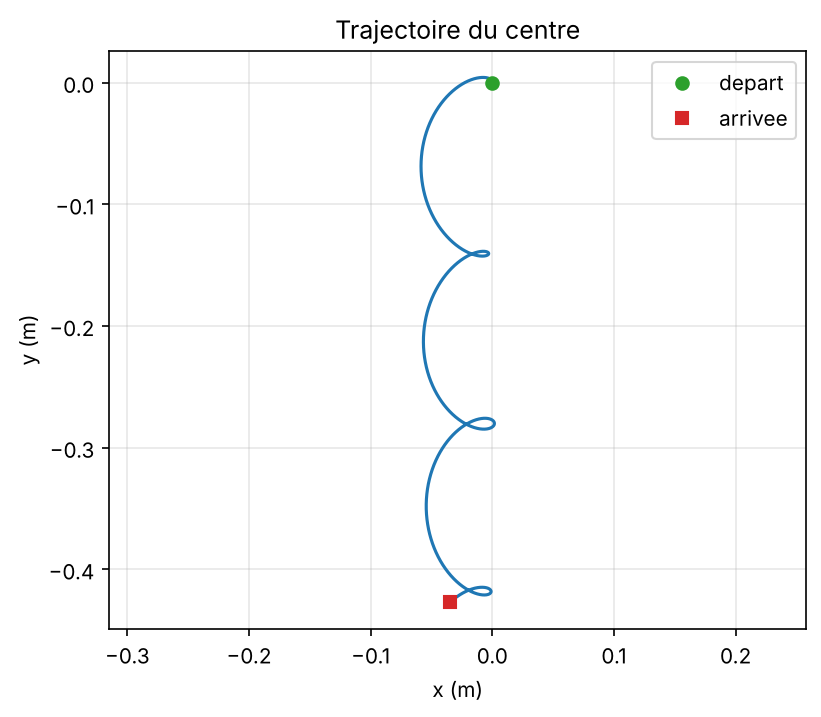
\includegraphics[width=\linewidth]{chapitre4/figures/case_a_trajectory.png}
        \caption{Trajectoire de $G$ dans le plan}
    \end{subfigure}
    \hfill
    \begin{subfigure}{0.52\textwidth}
        \centering
        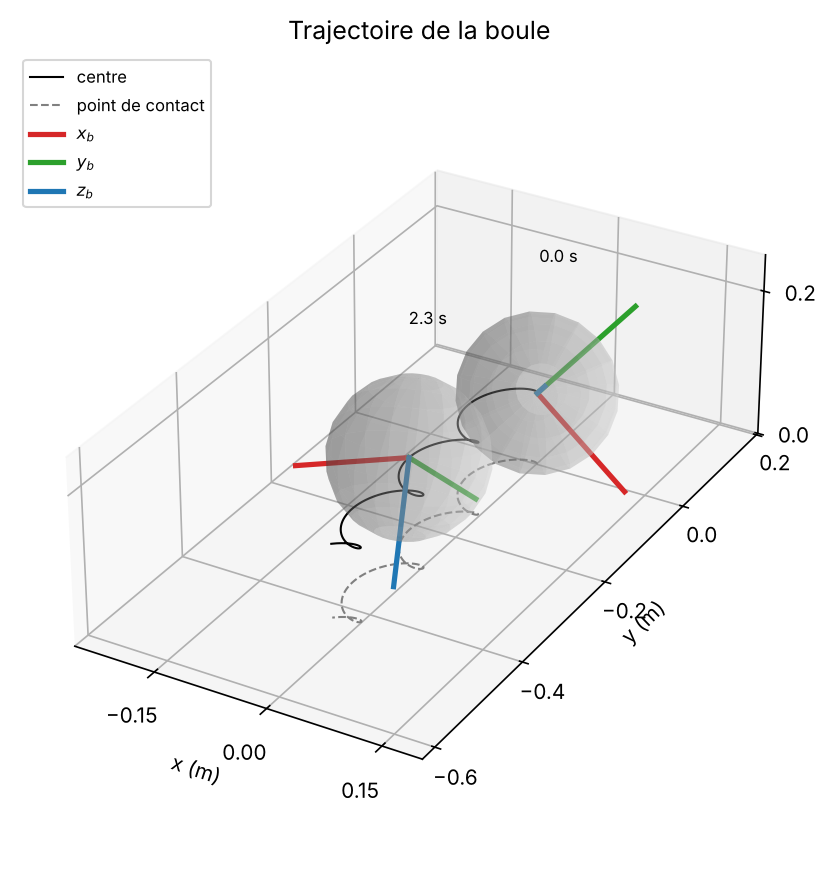
\includegraphics[width=\linewidth]{chapitre4/figures/case_a_trajectory_3d.png}
        \caption{Boule et axes du corps le long de la trajectoire}
    \end{subfigure}
    \caption{Boule anisotrope : trajectoire du centre $G$}
    \label{fig-traj-anisotrope}
\end{figure}

\begin{figure}[H]
    \centering
    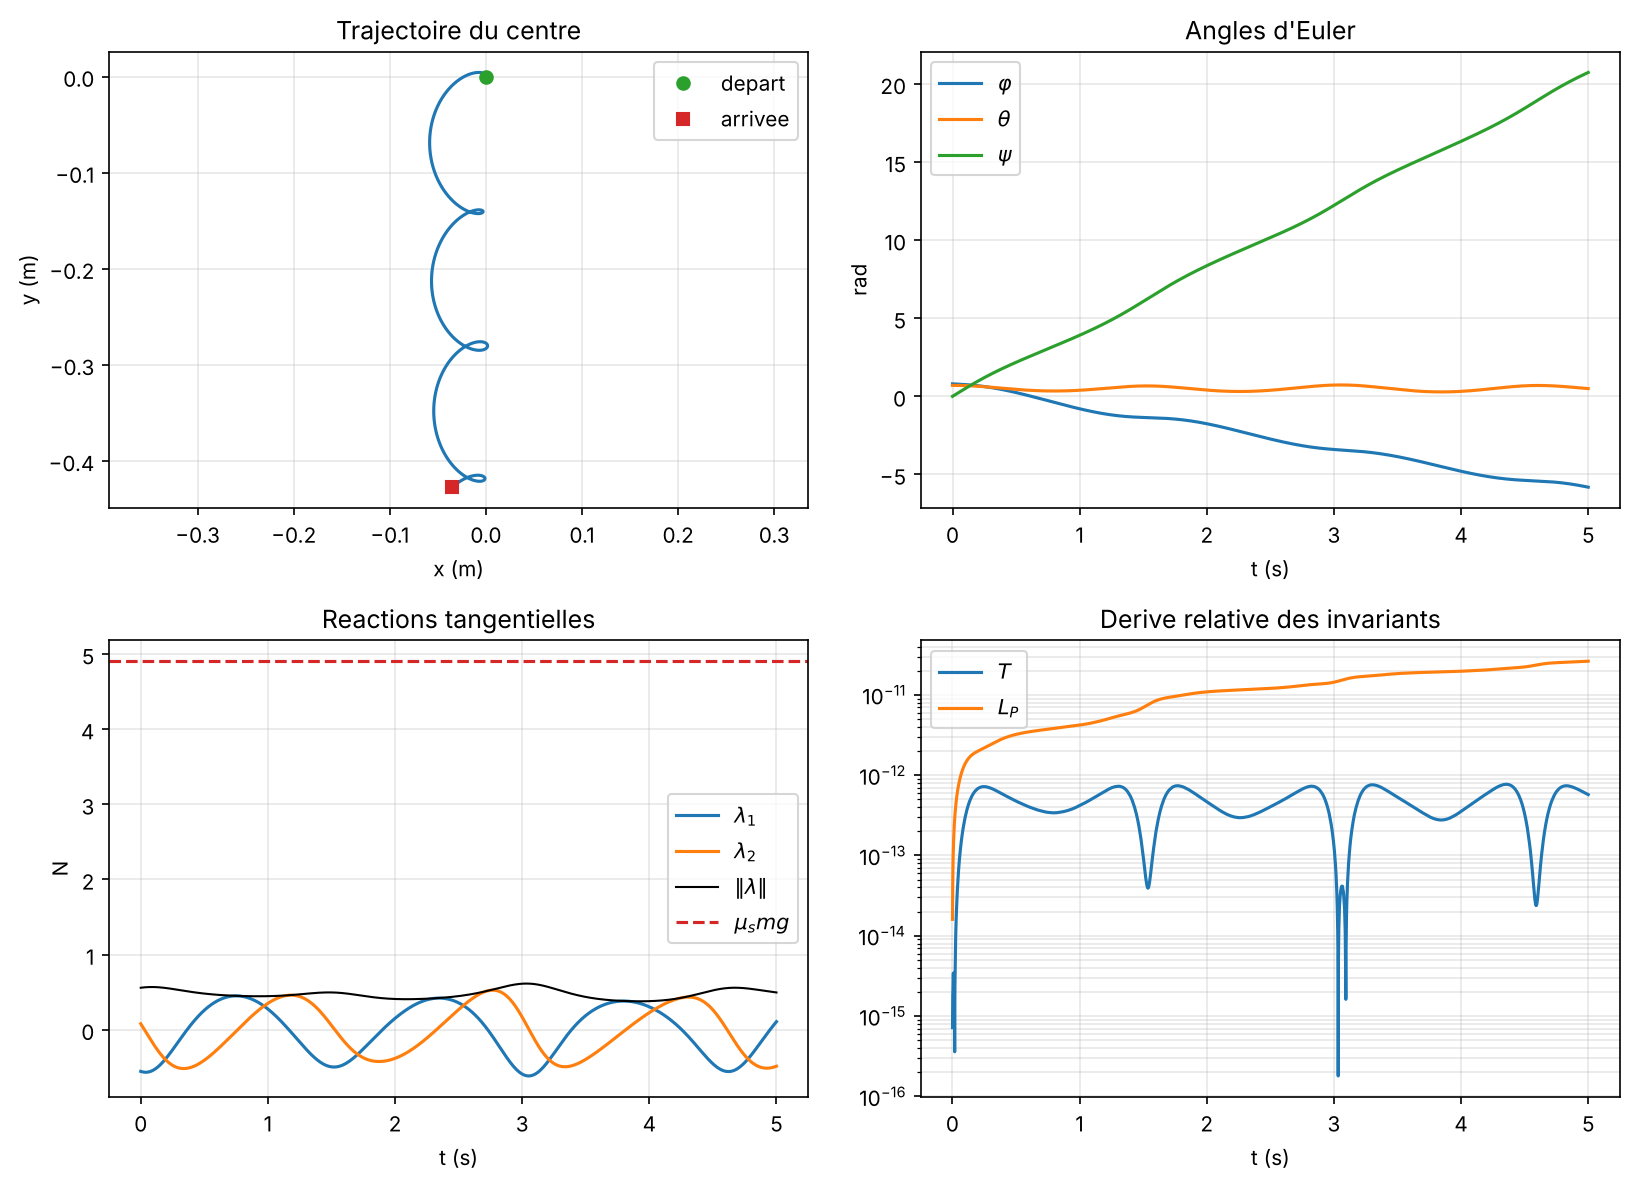
\includegraphics[width=0.9\textwidth]{chapitre4/figures/case_a_summary.png}
    \caption{Boule anisotrope : trajectoire, angles d'Euler, réactions
    tangentielles et dérive des invariants}
    \label{fig-resume-anisotrope}
\end{figure}

\textbf{Contrôles de la simulation :} Les hypothèses de validité sont vérifiées sur
toute la durée :
\begin{itemize}
    \item $|\cos\theta| \geq 0{,}75$ : les angles d'Euler restent loin
    de la singularité.
    \item $\|\vect{\lambda}_k\| \leq 0{,}62$ N $\ll \mu_s\,m\,g$ : pas de
    glissement, et $\mu_s \geq 0{,}07$ suffirait.
    \item Dérives relatives maximales : $8\cdot 10^{-13}$ pour $T$ et
    $3\cdot 10^{-11}$ pour $\vect{L}_P$.
\end{itemize}

% ----------------------------------------------------------------------------
\subsubsection{Boule isotrope}

On prend la boule homogène, $\mat{I}_b = \tfrac25\,m\,a^2\,\Id
= 4\cdot 10^{-3}\,\Id$ kg.m$^2$, avec le même lancer. C'est une sphère dont on connaît a priori la trajectoire, on l'utilise ici juste pour montrer la validité de la simulation.

\begin{proposition}[Boule isotrope]
    Si $\mat{I}_b = I_0\,\Id$, les frottements sont nuls,
    $\vect{\Omega}(t) = \vect{\Omega}_0$, et le centre suit un
    mouvement rectiligne uniforme
    \[
        r(t) = r_0 + a\,t\begin{pmatrix}
            \Omega_{0,y}\\ -\,\Omega_{0,x}
        \end{pmatrix}
    \]
\end{proposition}

\begin{demonstration}
    On note $\vect{F} = N_x\,\vect{e}_x + N_y\,\vect{e}_y$ le
    frottement en $P$. La vitesse du centre de masse s'écrit : 
    \[
        \vect{v}_G = a\,\vect{\Omega}\wedge\vect{e}_z
    \]
    La loi de Newton (ou le théorème de la quantité de mouvement) donne
    \[
        m\,\dot{\vect{v}}_G = \vect{F}
    \]
    Comme $\mat{I}_b = I_0\,\Id$, le moment cinétique en $G$ est
    $\vect{L}_G = I_0\,\vect{\Omega}$. Avec
    $\vect{GP} = -\,a\,\vect{e}_z$, le théorème du moment cinétique
    en $G$ donne
    \[
        I_0\,\dot{\vect{\Omega}}
        = -\,a\,\vect{e}_z\wedge\bigl(\vect{F} + N_z\,\vect{e}_z\bigr)
        = -\,a\,\vect{e}_z\wedge\vect{F}
    \]
    Or, on a : 
    \[
        \dot{\vect{v}}_G = a\,\dot{\vect{\Omega}}\wedge\vect{e}_z
        = -\,\frac{a^2}{I_0}\,(\vect{e}_z\wedge\vect{F})\wedge\vect{e}_z
    \]
    Comme $\vect{F}$ est horizontal,
    $(\vect{e}_z\wedge\vect{F})\wedge\vect{e}_z = \vect{F}$, donc
    \[
        \dot{\vect{v}}_G = -\,\frac{a^2}{I_0}\,\vect{F}
    \]
    En reinjectant dans la loi de Newton, on a :
    \[
        \Bigl(1 + \frac{m\,a^2}{I_0}\Bigr)\vect{F} = \vect{0} \longleftrightarrow \vect{F} = \vect{0}
    \]
    d'où $\vect{F} = \vect{0}$. On en déduit
    $\dot{\vect{\Omega}} = \vect{0}$ et $\dot{\vect{v}}_G = \vect{0}$,
    donc $\vect{v}_G = a\,\vect{\Omega}_0\wedge\vect{e}_z
    = a\,(\Omega_{0,y},\,-\,\Omega_{0,x},\,0)$.
\end{demonstration}

\begin{figure}[H]
    \centering
    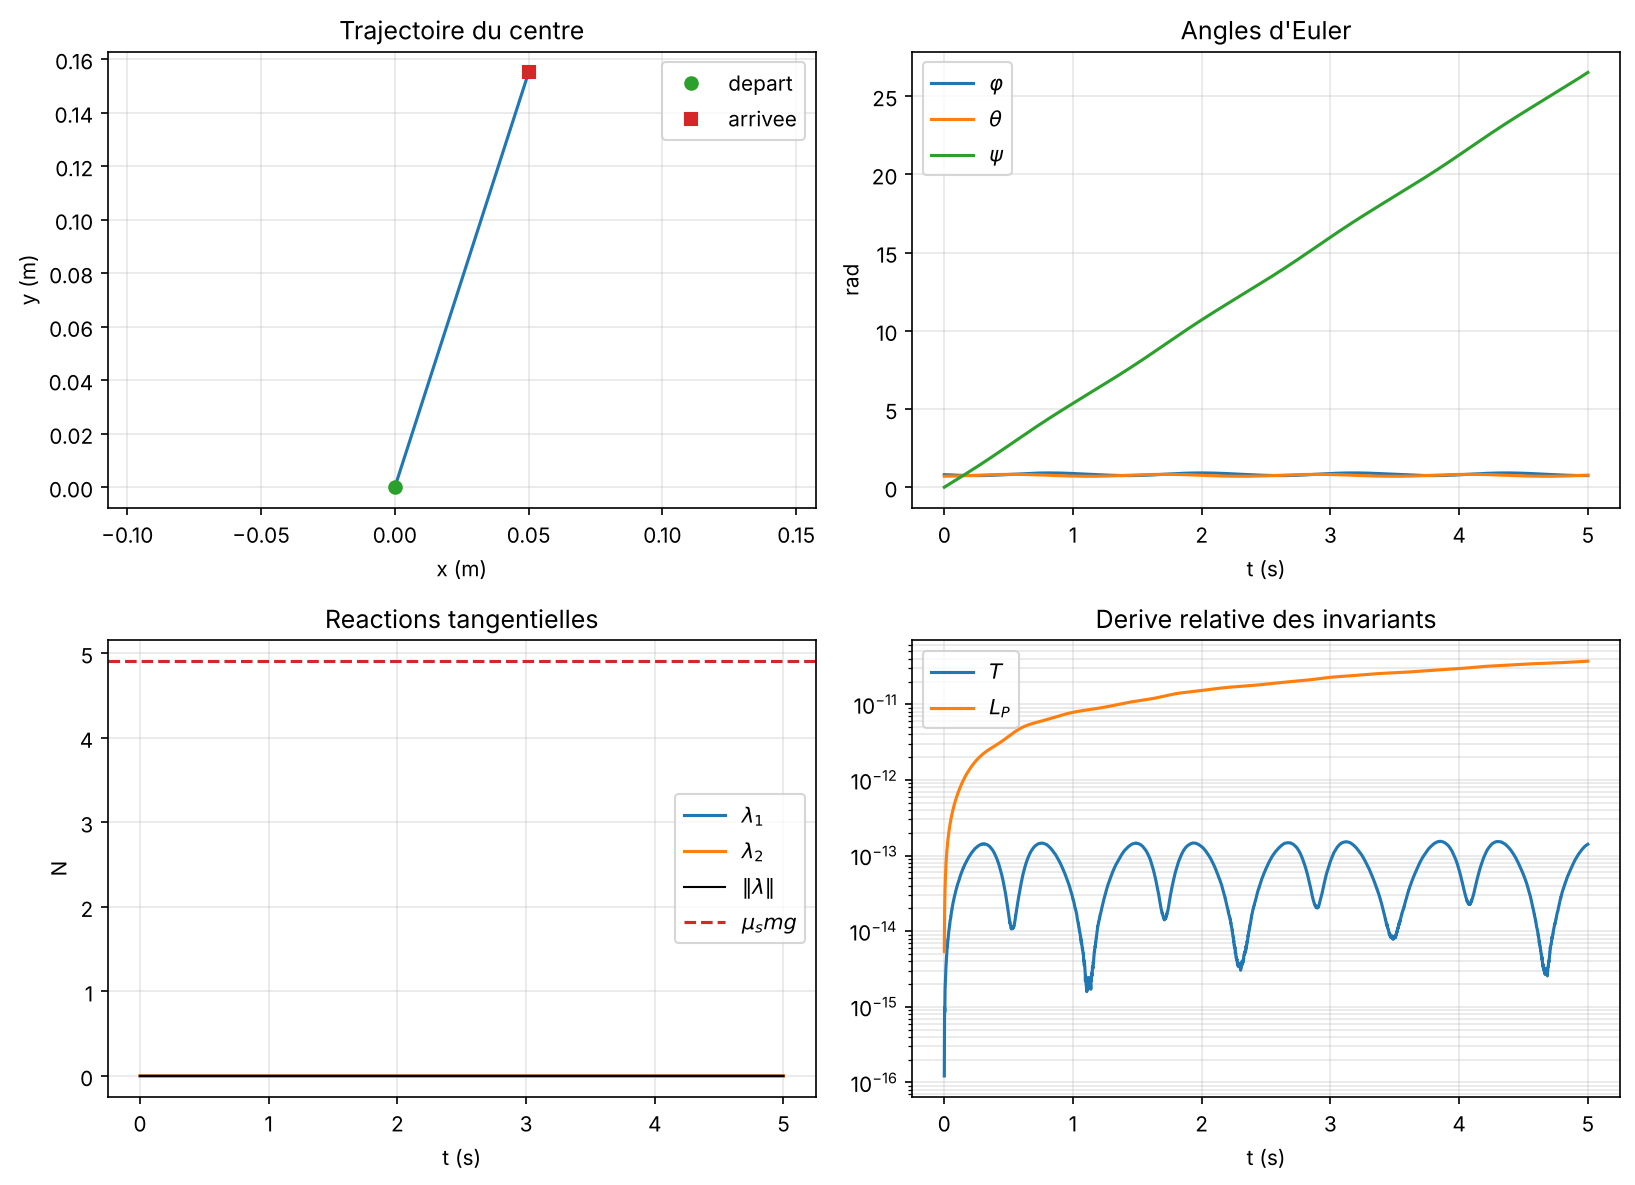
\includegraphics[width=0.9\textwidth]{chapitre4/figures/case_iso_summary.png}
    \caption{Boule isotrope : trajectoire, angles d'Euler, réactions
    tangentielles et dérive des invariants}
    \label{fig-resume-isotrope}
\end{figure}

La simulation retrouve cette solution avec (\cref{fig-resume-isotrope}) :
\[
    \max_k \|\vect{\Omega}_k - \vect{\Omega}_0\| \approx 6\cdot 10^{-11},
    \qquad
    \max_k \|r_k - r(t_k)\| \approx 1{,}5\cdot 10^{-11}\ \text{m},
    \qquad
    \max_k \|\vect{\lambda}_k\| \approx 10^{-16}\ \text{N}
\]
  % II.8. Résultats de la simulation
% ============================================================================
%  Chapitre 4, partie III : Algorithme de simulation en quaternions
% ============================================================================

% ----------------------------------------------------------------------------
\section{Algorithme de simulation - Orientation en quaternions}
% ----------------------------------------------------------------------------

La simulation en angles d'Euler ne tient que tant que
$|\cos\theta| > \varepsilon$. Dans cette partie, on garde la même
dynamique, mais on représente l'orientation par un quaternion unitaire
pour supprimer cette singularité.

% ----------------------------------------------------------------------------
\subsection{Motivation : problème du gimbal lock}

\subsubsection{Perte d'un degré de liberté}

Les colonnes de $\mat{E}$ donnent la vitesse angulaire produite par
chaque angle :
\[
    \pd{\vect{\omega}}{\dot\varphi} = \begin{pmatrix}
        1\\ 0\\ 0
    \end{pmatrix},
    \qquad
    \pd{\vect{\omega}}{\dot\theta} = \begin{pmatrix}
        0\\ c_\varphi\\ -s_\varphi
    \end{pmatrix},
    \qquad
    \pd{\vect{\omega}}{\dot\psi} = \begin{pmatrix}
        -s_\theta\\ s_\varphi c_\theta\\ c_\varphi c_\theta
    \end{pmatrix}
\]
Lorsque $\theta = \pm\pi/2$, la troisième colonne devient
$(\mp 1, 0, 0)$, colinéaire à la première : $\varphi$ et $\psi$
décrivent la même rotation. On perd un degré de liberté, et
$\det\mat{E} = \cos\theta = 0$.

\subsubsection{Conséquence pour la simulation}

La sphère, elle, peut toujours tourner autour de l'axe bloqué. Mais
pour décrire cette rotation en angles d'Euler, il faut
\[
    \dot\alpha = \mat{E}^{-1}\,\vect{\omega}
\]
dont les composantes sont en $1/\cos\theta$. Près de la singularité,
un petit mouvement selon l'axe bloqué donne donc des vitesses
$\dot\varphi$ et $\dot\psi$ très grandes, et des accélérations
$\ddot\alpha$ plus grandes encore. Le système réduit devient mal
conditionné, et le schéma RK4 à pas fixe perd sa précision. Cependant, le mouvement de la sphère n'a rien de particulier. La singularité vient uniquement de la représentation de l'orientation, pas de la physique. Il suffit donc de changer la représentation de l'orientation d'où la solution avec les quaternions.

\subsubsection{Solution par les quaternions}

Un quaternion unitaire $\quat{q}$ décrit l'orientation avec $4$
paramètres liés par $\|\quat{q}\| = 1$. La matrice de rotation
$\mat{R}(\quat{q})$ et la cinématique $\dot{\quat{q}} = \tfrac12\,\quat{q}\quatmul(0,\vect{\omega})$ sont définies pour toute orientation et il n'y a plus de
singularité. Le prix à payer est un paramètre redondant, et une
renormalisation de $\quat{q}$ au cours de la simulation, qui ne sont pas trop chers par rapport à la stabilité que l'on va gagner.

% ----------------------------------------------------------------------------
\subsection{Dynamique du système en représentation quaternionique}

\subsubsection{État}

\textbf{Quaternion des angles d'Euler : } Avec la définition de représentation quaternionique d'une rotation $\theta$ autour d'un axe unitaire $\vect{u}$ du chapitre 2, et avec la convention
$Z$-$Y'$-$X''$, le quaternion est
le produit des trois rotations élémentaires, dans le même ordre que
$\mat{R} = \mat{R}_z(\psi)\,\mat{R}_y(\theta)\,\mat{R}_x(\varphi)$ :
\[
    \quat{q}(\alpha)
    = \Bigl(\cos\tfrac{\psi}{2},\, 0,\, 0,\, \sin\tfrac{\psi}{2}\Bigr)
    \quatmul\Bigl(\cos\tfrac{\theta}{2},\, 0,\, \sin\tfrac{\theta}{2},\, 0\Bigr)
    \quatmul\Bigl(\cos\tfrac{\varphi}{2},\, \sin\tfrac{\varphi}{2},\, 0,\, 0\Bigr)
\]

On décrit l'orientation par $\quat{q}$ et la rotation par la vitesse
angulaire $\vect{\omega}$ exprimée dans le corps. L'état est ainsi 
\[
    Y = (\quat{q},\vect{\omega})\in\R^7, \quad \text{avec} \quad \|\quat{q}\| = 1
\]
soit $7$ nombres pour $6$ degrés de liberté. Comme démontré plus haut avec les angles d'Euler, on peut calculer la position à part. On cherche donc seulement à écrire
\[
    \dot Y = \begin{pmatrix}
        \dot{\quat{q}}\\ \dot{\vect{\omega}}
    \end{pmatrix}
    = \begin{pmatrix}
        \tfrac12\,\quat{q}\quatmul(0,\vect{\omega})\\
        \dot{\vect{\omega}}
    \end{pmatrix}
\]
La première composante est la cinématique quaternionique. Il nous reste à trouver l'équation de $\dot{\vect{\omega}}$.

\subsubsection{Équation de \texorpdfstring{$\dot{\vect{\omega}}$}{omega point}}
Il suffit ici d'utiliser les équations de Gibbs-Appell avec $\vect{\omega}$ comme
pseudo-vitesses.
D'abord, il nous faut retrouver la fonction de Gibbs-Appell en fonction de $\vect{\omega}$.
Soit $\vect{\gamma}$ l'axe vertical vu depuis le corps, $\vect{\gamma}$ s'écrit ainsi dans le repère corps :
\[
    \vect{\gamma} = \mat{R}(\quat{q})^T\vect{e}_z
\]
D'après la fonction de Gibbs-Appell d'un solide, à des termes sans $\dot{\vect{\omega}}$ près, on a :
\[
    \mathcal{G} = \frac{1}{2}\,m\,\|\vect{a}_G\|^2
    + \frac{1}{2}\,\dot{\vect{\omega}}^T\mat{I}_b\,\dot{\vect{\omega}}
    + \dot{\vect{\omega}}\cdot\bigl(\vect{\omega}\wedge
    \mat{I}_b\vect{\omega}\bigr)
\]
On voit que le seul terme qu'il reste à calculer est $\vect{a}_G$.

\textbf{Dérivées de $\mat{R}$ et $\vect{\gamma}$ : } Comme
$\vect{\Omega} = \mat{R}\,\vect{\omega}$,
\[
    \dot{\mat{R}} = \hatx{\vect{\Omega}}\,\mat{R}
    = \mat{R}\,\hatx{\vect{\omega}}
\]
et comme $\vect{e}_z$ est fixe,
\[
    \dot{\vect{\gamma}} = \dot{\mat{R}}^T\vect{e}_z
    = -\,\hatx{\vect{\omega}}\,\mat{R}^T\vect{e}_z
    = -\,\vect{\omega}\wedge\vect{\gamma}
    = \vect{\gamma}\wedge\vect{\omega}
\]

\textbf{Accélération du centre : } D'après le roulement, avec
$\vect{\Omega} = \mat{R}\,\vect{\omega}$ et
$\vect{e}_z = \mat{R}\,\vect{\gamma}$, on a :
\[
    \vect{v}_G = a\,\vect{\Omega}\wedge\vect{e}_z
    = a\,\mat{R}\vect{\omega}\wedge\mat{R}\vect{\gamma}
\]
puis, comme une rotation conserve le produit vectoriel,
\[
    \vect{v}_G = a\,\mat{R}\,(\vect{\omega}\wedge\vect{\gamma})
\]
En dérivant ce terme, on a l'accélération :
\[
    \vect{a}_G = a\,\mat{R}\Bigl(
    \vect{\omega}\wedge(\vect{\omega}\wedge\vect{\gamma})
    + \dot{\vect{\omega}}\wedge\vect{\gamma}
    + \vect{\omega}\wedge(\vect{\gamma}\wedge\vect{\omega})\Bigr)
\]
Le premier et le dernier terme s'annulent, car
$\vect{\omega}\wedge\vect{\gamma} + \vect{\gamma}\wedge\vect{\omega}
= \vect{0}$, d'où
\[
    \vect{a}_G = a\,\mat{R}\,(\dot{\vect{\omega}}\wedge\vect{\gamma})
\]
Comme $\mat{R}$ conserve la norme,
$\|\vect{a}_G\| = a\,\|\dot{\vect{\omega}}\wedge\vect{\gamma}\|$.

\begin{proposition}[Fonction de Gibbs-Appell de la sphère avec $\vect{\omega}$ comme pseudo-vitesse]
    Avec $\vect{\omega}$ comme pseudo-vitesse, la fonction de
    Gibbs-Appell de la sphère s'écrit :
    \[
        \mathcal{G} = \tfrac12\,m\,a^2\,
        \|\dot{\vect{\omega}}\wedge\vect{\gamma}\|^2
        + \tfrac12\,\dot{\vect{\omega}}^T\mat{I}_b\,\dot{\vect{\omega}}
        + \dot{\vect{\omega}}\cdot(\vect{\omega}\wedge\mat{I}_b\,
        \vect{\omega})
    \]
\end{proposition}
Ensuite, on développe le premier terme en utilisant la formule de la
norme d'un produit vectoriel
$\|\vect{u}\wedge\vect{v}\|^2 = \|\vect{u}\|^2\,\|\vect{v}\|^2
- (\vect{u}\cdot\vect{v})^2$ avec $\|\vect{\gamma}\| = 1$ :
\[
    \|\dot{\vect{\omega}}\wedge\vect{\gamma}\|^2
    = \|\dot{\vect{\omega}}\|^2
    - (\dot{\vect{\omega}}\cdot\vect{\gamma})^2
    = \dot{\vect{\omega}}^T\bigl(\Id - \vect{\gamma}\vect{\gamma}^T
    \bigr)\dot{\vect{\omega}}
\]
On réécrit la fonction de Gibbs-Appell sous la forme :
\[
    \mathcal{G} = \tfrac12\,\dot{\vect{\omega}}^T\mat{K}(\vect{\gamma})
    \,\dot{\vect{\omega}}
    + \dot{\vect{\omega}}\cdot(\vect{\omega}\wedge\mat{I}_b\,
    \vect{\omega}) \quad \text{avec} \quad
    \mat{K}(\vect{\gamma}) = \mat{I}_b
    + m\,a^2\,\bigl(\Id - \vect{\gamma}\vect{\gamma}^T\bigr)
\]
Le potentiel $V = m g a$ est constant et aucune force non
conservative n'est appliquée, donc $\mathcal{Q} = 0$. On en déduit
l'équation de Gibbs-Appell :
\[
    \pd{\mathcal{G}}{\dot{\vect{\omega}}}
    = \mat{K}(\vect{\gamma})\,\dot{\vect{\omega}}
    + \vect{\omega}\wedge\mat{I}_b\,\vect{\omega} = \vect{0}
\]
\begin{proposition}[Inversibilité de $\mat{K}(\vect{\gamma})$]
    La matrice $\mat{K}(\vect{\gamma})$ est symétrique, définie positive donc inversible.
\end{proposition}
\begin{demonstration}
    On voit bien que $\mat{K}(\vect{\gamma})$ est symétrique,
    et pour tout $\vect{v}\neq\vect{0}$,
    \[
        \vect{v}^T\mat{K}(\vect{\gamma})\,\vect{v}
        = \vect{v}^T\mat{I}_b\,\vect{v}
        + m\,a^2\,\|\vect{v}\wedge\vect{\gamma}\|^2
        \geq \vect{v}^T\mat{I}_b\,\vect{v} > 0
    \]
    car $\mat{I}_b$ est définie positive. $\mat{K}$ est donc inversible.
\end{demonstration}

\begin{proposition}[Dynamique en quaternions]
    Avec
    \[
        \mat{K}(\vect{\gamma}) = \mat{I}_b
        + m\,a^2\,\bigl(\Id - \vect{\gamma}\vect{\gamma}^T\bigr)
    \]
    on a
    \[
        \mat{K}(\vect{\gamma})\,\dot{\vect{\omega}}
        = -\,\vect{\omega}\wedge\mat{I}_b\,\vect{\omega}
    \]
\end{proposition}

On a donc la dynamique
\[
    \dot Y = f(Y)= \begin{pmatrix}
        \tfrac12\,\quat{q}\quatmul(0,\vect{\omega})\\
        -\,\mat{K}(\vect{\gamma})^{-1}
        \bigl(\vect{\omega}\wedge\mat{I}_b\,\vect{\omega}\bigr)
    \end{pmatrix}
\]
définie pour toute orientation, sans condition sur $\cos\theta$.

\subsubsection{Position et frottements}

Une fois $Y$ connu, la position et les frottements s'en déduisent sans
nouvelle équation. On repasse dans le repère du sol avec
$\vect{\Omega} = \mat{R}\,\vect{\omega}$. On a, avec
$\dot{\mat{R}} = \mat{R}\,\hatx{\vect{\omega}}$,
\[
    \dot{\vect{\Omega}} = \mat{R}\,(\vect{\omega}\wedge\vect{\omega})
    + \mat{R}\,\dot{\vect{\omega}}
    = \mat{R}\,\dot{\vect{\omega}}
\]

\textbf{Position : }
\[
    \dot{\vect{r}} = \vect{v}_G = \begin{pmatrix}
        \dot x\\ \dot y\\ 0
    \end{pmatrix}
    = a\,\vect{\Omega}\wedge\vect{e}_z
    = a\begin{pmatrix}
        \Omega_y\\ -\,\Omega_x\\ 0
    \end{pmatrix}
\]
On peut simplement calculer $\vect{r}$ avec une quadrature. 

\textbf{Frottements : } D'après la loi de Newton en $x$ et $y$,
$(N_x, N_y, 0) = m\,\vect{a}_G$. Avec
$\vect{a}_G = a\,\mat{R}\,(\dot{\vect{\omega}}\wedge\vect{\gamma})$ et
$\mat{R}\,\vect{\gamma} = \vect{e}_z$ : 
\[
    \vect{a}_G = a\,\dot{\vect{\Omega}}\wedge\vect{e}_z
    = a\begin{pmatrix}
        \dot\Omega_y\\ -\,\dot\Omega_x\\ 0
    \end{pmatrix}
\]

\begin{proposition}[Position et frottements]
    Avec $\vect{\Omega} = \mat{R}(\quat{q})\,\vect{\omega}$ et
    $\dot{\vect{\Omega}} = \mat{R}(\quat{q})\,\dot{\vect{\omega}}$,
    \[
        \dot x = a\,\Omega_y,
        \qquad
        \dot y = -\,a\,\Omega_x,
        \qquad
        N_x = m\,a\,\dot\Omega_y,
        \qquad
        N_y = -\,m\,a\,\dot\Omega_x
    \]
    et $N_z = m g$. Le non-glissement se vérifie a posteriori par
    \[
        \sqrt{N_x^2 + N_y^2} \leq \mu_s\,m\,g
    \]
\end{proposition}

% ----------------------------------------------------------------------------
\subsection{Schéma numérique}

On reprend le schéma RK4 de la partie II pour $\dot Y = f(Y)$, mais
cette fois-ci $Y = (\quat{q},\vect{\omega})$. La seule nouveauté est la
renormalisation de $\quat{q}$ à chaque pas.

\subsubsection{Conditions initiales}

\begin{proposition}[Conditions initiales]
    Les conditions initiales de cette dynamique sont
    $(r_0, \quat{q}(0), \vect{\omega}_0)$.
\end{proposition}

Comme en partie II, on se donne la position $r_0$, l'orientation
$\alpha_0$ et la vitesse angulaire $\vect{\Omega}_0$ dans $\rep{s}$.
On en déduit
\[
    \quat{q}(0) = \quat{q}(\alpha_0),
    \qquad
    \vect{\omega}_0 = \mat{R}\bigl(\quat{q}(0)\bigr)^T\vect{\Omega}_0
\]
Contrairement aux angles d'Euler, il n'y a aucune condition sur
$\cos\theta_0$ : on n'inverse plus $\mat{E}_s$. Enfin,
$\dot{\vect{\omega}}_0$ et les frottements initiaux s'obtiennent en
faisant les mêmes calculs que les étapes 3 et 4.

\subsubsection{Choix du pas}

\subsubsection{Schéma RK4 pour simuler le système}

\paragraph{Étape 1 : Orientation} Avec
$Y_k = (\quat{q}_k,\vect{\omega}_k)$, on évalue $f$ en quatre états
intermédiaires du pas,
\[
    Y^{(1)} = Y_k,
    \qquad
    Y^{(2)} = Y_k + \tfrac{h}{2}\,\vect{p}_1,
    \qquad
    Y^{(3)} = Y_k + \tfrac{h}{2}\,\vect{p}_2,
    \qquad
    Y^{(4)} = Y_k + h\,\vect{p}_3
\]
où $Y^{(i)} = (\quat{q}^{(i)},\vect{\omega}^{(i)})$ et
\[
    \vect{p}_i = f\bigl(Y^{(i)}\bigr)
    = \begin{pmatrix}
        \dot{\quat{q}}^{(i)}\\ \dot{\vect{\omega}}^{(i)}
    \end{pmatrix},
    \qquad
    \dot{\quat{q}}^{(i)} = \tfrac12\,\quat{q}^{(i)}\quatmul
    (0,\vect{\omega}^{(i)})
\]
avec
\[
    \mat{K}\bigl(\vect{\gamma}^{(i)}\bigr)\,\dot{\vect{\omega}}^{(i)}
    = -\,\vect{\omega}^{(i)}\wedge\mat{I}_b\,\vect{\omega}^{(i)},
    \qquad
    \vect{\gamma}^{(i)} = \mat{R}\bigl(\quat{q}^{(i)}\bigr)^T\vect{e}_z
\]
On obtient alors le nouvel état :
\[
    \quat{q}_{k+1} = \quat{q}_k + \tfrac{h}{6}\,\bigl(\dot{\quat{q}}^{(1)}
    + 2\,\dot{\quat{q}}^{(2)} + 2\,\dot{\quat{q}}^{(3)}
    + \dot{\quat{q}}^{(4)}\bigr),
    \qquad
    \vect{\omega}_{k+1} = \vect{\omega}_k + \tfrac{h}{6}\,\bigl(
    \dot{\vect{\omega}}^{(1)} + 2\,\dot{\vect{\omega}}^{(2)}
    + 2\,\dot{\vect{\omega}}^{(3)} + \dot{\vect{\omega}}^{(4)}\bigr)
\]

\paragraph{Étape 2 : Renormalisation} La dynamique conserve
$\|\quat{q}\| = 1$, mais pas le schéma : l'erreur est en
$O(h^5)$ sur un pas et s'accumule au cours de la simulation. Il nous faut alors 
renormaliser à chaque pas : 
\[
    \quat{q}_{k+1} \longleftarrow
    \frac{\quat{q}_{k+1}}{\|\quat{q}_{k+1}\|}
\]
L'écart $\bigl|\,\|\quat{q}_{k+1}\| - 1\,\bigr|$ avant renormalisation
reste de l'ordre de l'erreur du schéma.

\paragraph{Étape 3 : Accélération} On résout l'équation de
$\dot{\vect{\omega}}$ au nouvel état :
\[
    \mat{K}(\vect{\gamma}_{k+1})\,\dot{\vect{\omega}}_{k+1}
    = -\,\vect{\omega}_{k+1}\wedge\mat{I}_b\,\vect{\omega}_{k+1},
    \qquad
    \vect{\gamma}_{k+1} = \mat{R}(\quat{q}_{k+1})^T\vect{e}_z
\]
C'est la seconde moitié de $f(Y_{k+1})$, réutilisée comme
$\vect{p}_1$ au pas suivant.

\paragraph{Étape 4 : Position et frottements} En parallèle avec
l'étape 1, on calcule des poids RK4 pour $r$ avec
$\vect{g}_i = a\,\bigl(\Omega_y^{(i)}, -\,\Omega_x^{(i)}\bigr)$ et
$\vect{\Omega}^{(i)} = \mat{R}\bigl(\quat{q}^{(i)}\bigr)\,
\vect{\omega}^{(i)}$, tels que :
\[
    r_{k+1} = r_k + \tfrac{h}{6}\,\bigl(\vect{g}_1 + 2\,\vect{g}_2
    + 2\,\vect{g}_3 + \vect{g}_4\bigr)
\]
puis, avec $\dot{\vect{\Omega}}_{k+1} = \mat{R}(\quat{q}_{k+1})\,
\dot{\vect{\omega}}_{k+1}$,
\[
    N_{x,k+1} = m\,a\,\dot\Omega_{y,k+1},
    \qquad
    N_{y,k+1} = -\,m\,a\,\dot\Omega_{x,k+1}
\]

% ----------------------------------------------------------------------------
\subsection{Architecture de la simulation}

Voici l'architecture de la simulation prête à implémenter avec
l'orientation représentée par un quaternion unitaire.

\begin{figure}[H]
    \centering
    \begin{tikzpicture}[>=Stealth,
        bloc/.style={draw, thick, rounded corners=2pt, align=center,
            fill=coulprop!6, draw=coulprop, inner sep=4pt,
            font=\small},
        ctrl/.style={bloc, fill=couldef!8, draw=couldef},
        stop/.style={bloc, fill=coulthm!8, draw=coulthm},
        es/.style={bloc, fill=gray!8, draw=gray},
        fl/.style={->, thick},
        lab/.style={font=\footnotesize, fill=white, inner sep=1pt}]

        \node[es] (in) at (0,0) {Entrées : $m$, $a$, $\mat{I}_b$,
            $\mu_s$ ; $r_0$, $\alpha_0$, $\vect{\Omega}_0$ ; $h$, $N$};
        \node[bloc] (init) at (0,-1.3)
            {Initialisation : $\quat{q}(0) = \quat{q}(\alpha_0)$,
            \quad $\vect{\omega}_0 = \mat{R}\bigl(\quat{q}(0)\bigr)^T
            \vect{\Omega}_0$, \quad
            $Y_0 = \bigl(\quat{q}(0),\vect{\omega}_0\bigr)$};
        \node[bloc] (f) at (0,-3.3)
            {Évaluation de $f$ en $Y^{(i)}$, $i = 1,\dots,4$ :\\[2pt]
            $\dot{\quat{q}}^{(i)} = \tfrac12\,\quat{q}^{(i)}\quatmul
            (0,\vect{\omega}^{(i)})$\\[2pt]
            $\mat{R}\bigl(\quat{q}^{(i)}\bigr)$
            $\;\to\;$ $\vect{\gamma}^{(i)}$
            $\;\to\;$ $\mat{K}\bigl(\vect{\gamma}^{(i)}\bigr)\,
            \dot{\vect{\omega}}^{(i)}
            = -\,\vect{\omega}^{(i)}\wedge\mat{I}_b\,\vect{\omega}^{(i)}$};
        \node[bloc] (rk) at (-2.9,-5.5)
            {Étape 1 : $Y_{k+1}$ par RK4\\[2pt]
            Étape 2 : $\quat{q}_{k+1} \leftarrow
            \quat{q}_{k+1}/\|\quat{q}_{k+1}\|$\\[2pt]
            Étape 3 : $\dot{\vect{\omega}}_{k+1}$};
        \node[bloc] (rl) at (2.9,-5.5)
            {Étape 4 : $r_{k+1}$ avec les $\vect{g}_i$,\\[2pt]
            $N_{x,k+1}$, $N_{y,k+1}$};
        \node[ctrl] (c) at (0,-7.4)
            {Contrôles : $T$, $\vect{L}_P$ conservés ;
            $\sqrt{N_{x,k+1}^2 + N_{y,k+1}^2} \leq \mu_s\,m\,g$};
        \node[stop] (arret) at (-3.6,-9.3)
            {Arrêt : simulation\\non valide};
        \node[es] (out) at (3.6,-9.3)
            {Sorties : $r_k$, $\quat{q}_k$, $\vect{\omega}_k$,
            $(N_x, N_y)_k$,\\
            $k = 0,\dots,N$};

        \draw[fl] (in) -- (init);
        \draw[fl] (init) -- (f);
        \draw[fl] (f) -- (rk);
        \draw[fl] (f) -- (rl);
        \draw[fl] (rk) -- (c);
        \draw[fl] (rl) -- (c);
        \draw[fl, coulthm] (c) -- node[lab, pos=0.45, left=2pt]
            {non} (arret);
        \draw[fl] (c) -- node[lab, pos=0.45, right=2pt]
            {oui, $k = N$} (out);
        \coordinate (droite) at (6.4,0);
        \draw[fl] (c.east) -- (c.east -| droite) -- (f.east -| droite)
            node[lab, pos=0.5, left=2pt, align=right]
            {oui,\\$k \leftarrow k+1$} -- (f.east);

        \begin{scope}[on background layer]
            \node[draw=gray, dashed, rounded corners, inner sep=7pt,
                fit=(f) (rk) (rl) (c) (c.east -| droite)] (boucle) {};
        \end{scope}
        \node[font=\footnotesize, gray, anchor=south west]
            at (boucle.north west) {boucle sur $k$};
    \end{tikzpicture}
    \caption{Architecture de la simulation de la sphère de Chaplygin
    en quaternions}
\end{figure}

Par rapport aux angles d'Euler, le contrôle $|\cos\theta| > \varepsilon$
disparaît, et l'étape de renormalisation s'ajoute.

\subsection{Validation de la simulation}
\subsubsection{Écart avec le modèle en angles d'Euler}

On relance la boule anisotrope de la partie précédente
(figure~\ref{fig-traj-anisotrope}), avec les mêmes paramètres et le même
pas $h$, une fois avec le modèle en angles d'Euler et une fois avec le
modèle en quaternions. Sur ce lancer, $|\cos\theta| \geq 0{,}74$ et les deux modèles décrivent la même
dynamique. Les deux simulations doivent donc donner le même résultat, à l'erreur du schéma près.
\paragraph{Écarts mesurés : } on note avec un indice $E$ (resp. $Q$) les
grandeurs calculées en angles d'Euler (resp. en quaternions), et on
mesure à chaque pas
\[
    \|r_k^E - r_k^Q\|,
    \qquad
    \|\mat{R}_k^E - \mat{R}_k^Q\|_F,
    \qquad
    \|(N_x, N_y)_k^E - (N_x, N_y)_k^Q\|
\]
où $\|\cdot\|_F$ est la norme de Frobenius. Sur les $5$ s de simulation,
ces écarts restent inférieurs à $1{,}1\cdot 10^{-11}$ m,
$2{,}2\cdot 10^{-11}$ et $6{,}7\cdot 10^{-12}$ N respectivement
(figure~\ref{fig-ecart-euler-quat}). La dérive relative de l'énergie
reste de l'ordre de $10^{-12}$ pour les deux modèles.

\begin{figure}[H]
    \centering
    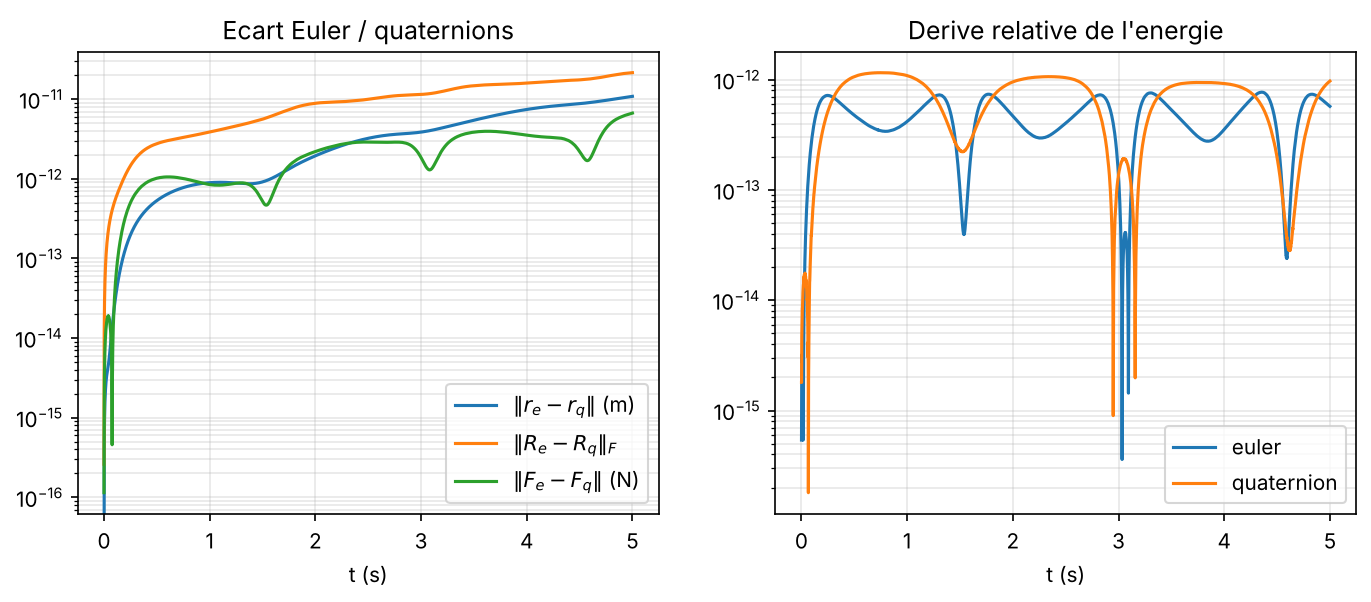
\includegraphics[width=0.95\textwidth]{chapitre4/figures/validation_case_a_errors.png}
    \caption{Boule anisotrope : écart entre les simulations en angles
    d'Euler et en quaternions, et dérive relative de l'énergie}
    \label{fig-ecart-euler-quat}
\end{figure}

Loin de la singularité, la simulation en quaternions redonne donc les
résultats de la simulation en angles d'Euler.

\paragraph{Près du gimbal lock}

On lance maintenant la même boule avec un tangage proche de $90^\circ$ :
\[
    \alpha_0 = (0;\ 90^\circ - 0{,}4^\circ;\ 0),
    \qquad
    \vect{\Omega}_0 = (5;\ 1;\ 2) \text{ rad.s}^{-1}
\]
avec le même pas $h$ et la même durée. On peut par partir de gimbal lock car la simulation en angles d'Euler ne pourrait pas se lancer, mais on peut partir de son voisinage et lui donne de la vitesse pour atteindre gimbal lock.

\textbf{Trajectoire et angles : } les deux simulations coïncident jusqu'à
$t \approx 1{,}84$ s (figure~\ref{fig-gimbal-traj}). Les angles calculés en angles d'Euler s'écartent alors de ceux calculés en quaternions, et la trajectoire de $G$ avec eux :
l'écart atteint $50$ cm à $t = 5$ s.

\begin{figure}[H]
    \centering
    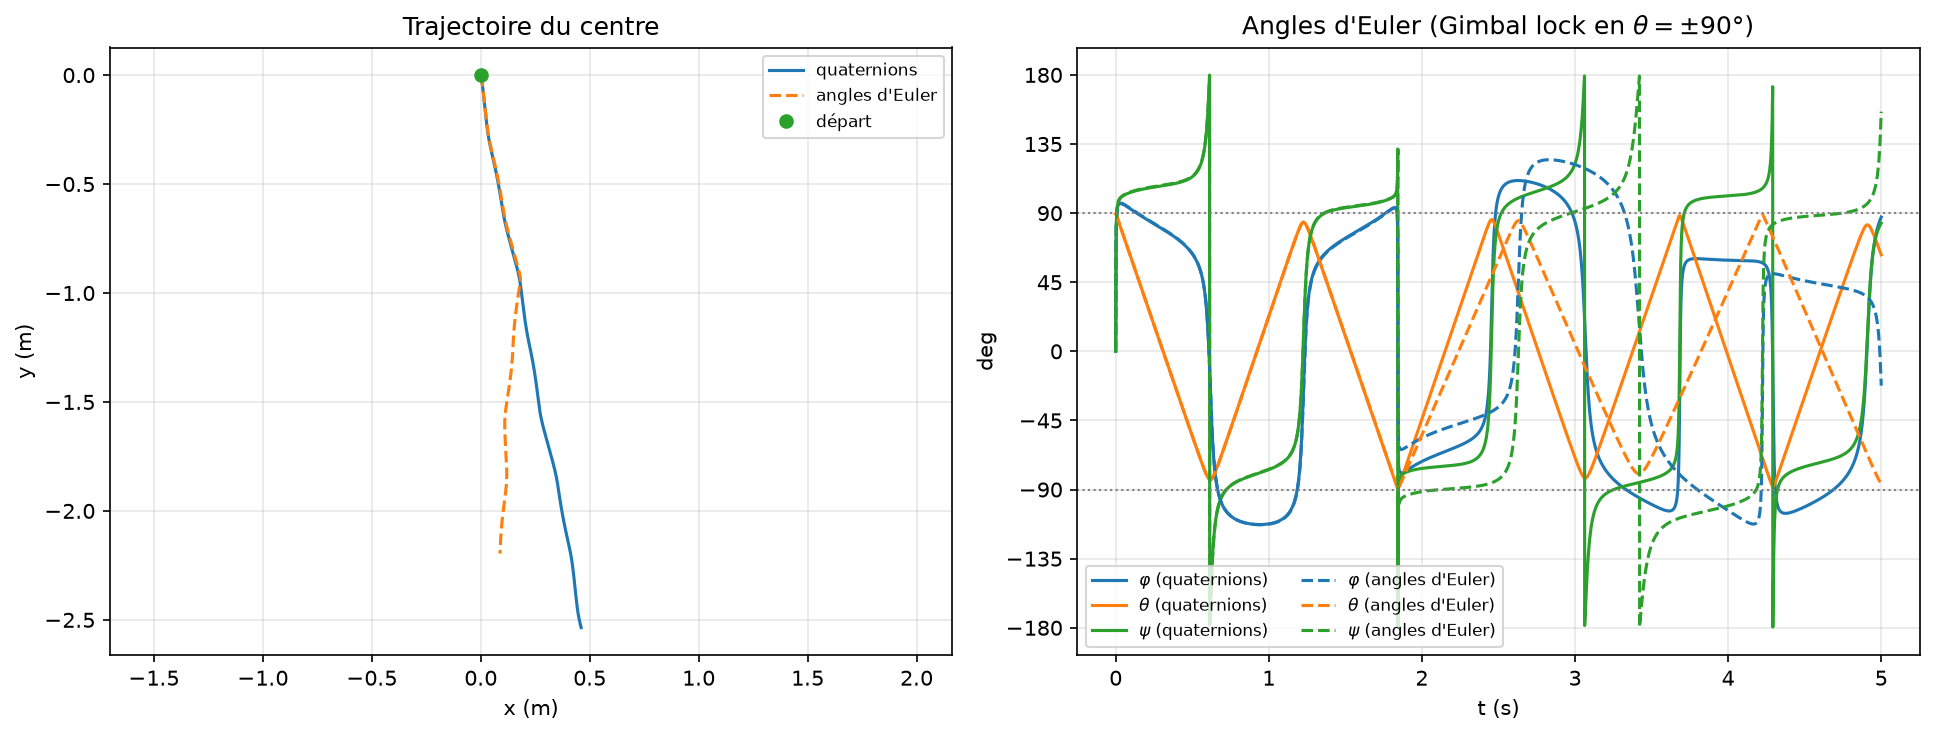
\includegraphics[width=\textwidth]{chapitre4/figures/case_b_euler_vs_quat.png}
    \caption{Près du gimbal lock : trajectoire de $G$ et angles d'Euler,
    calculés en quaternions (trait plein) et en angles d'Euler (tirets)}
    \label{fig-gimbal-traj}
\end{figure}

\textbf{Contrôles : } en quaternions, les dérives relatives de $T$ et de
$\vect{L}_P$ restent de l'ordre de $10^{-12}$
(figure~\ref{fig-gimbal-controles}). En angles d'Euler, les dérives de
$T$ et de $\vect{L}_P$ valent déjà quelques $10^{-3}$ dès le premier pas,
puisqu'on part près de la singularité, puis sautent à $43\ \%$ et
$33\ \%$ au passage de $t \approx 1{,}84$ s. L'erreur du schéma utilisant les angles d'Euler s'accumule dès les premiers pas près de la singularité, donc, pour la trajectoire, ce n'est pas forcément fiable pour la simulation en angles d'Euler.

En revanche, les deux autres contrôles passent : on a toujours
$|\cos\theta| > \varepsilon = 10^{-3}$, et
$\|(N_x, N_y)\| \leq 0{,}47$ N reste loin de $\mu_s\,m\,g \approx 4{,}9$ N.
La simulation en angles d'Euler est donc déclarée valide alors qu'elle
est fausse, on ne peut voir les erreurs qu'à travers les conservations.

\begin{figure}[H]
    \centering
    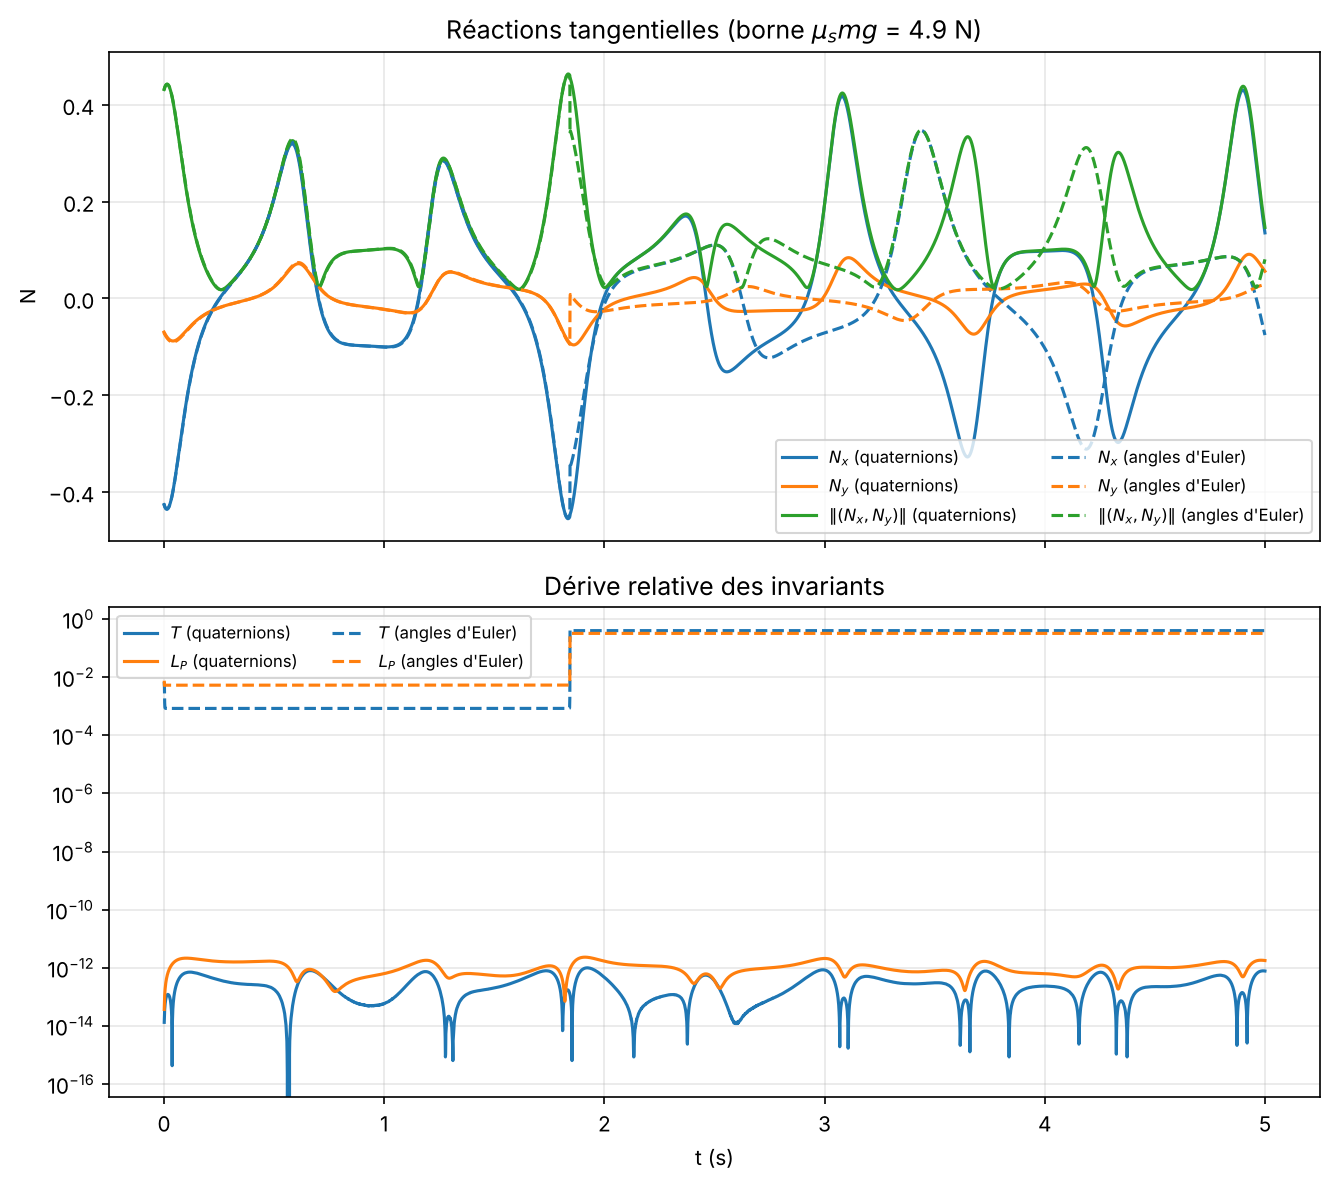
\includegraphics[width=0.8\textwidth]{chapitre4/figures/case_b_controls.png}
    \caption{Près du gimbal lock : réactions tangentielles et dérive
    relative des invariants, en quaternions (trait plein) et en angles
    d'Euler (tirets)}
    \label{fig-gimbal-controles}
\end{figure}

Près de la singularité, seule la simulation en quaternions reste fiable.
 % III. Algorithme de simulation en quaternions

% Parties suivantes, à discuter :
% \input{chapitre4/derive}      % III. Dérive de la contrainte
% \input{chapitre4/validation}  % IV.  Validation et résultats
